\documentclass{report}
%%% Import Packages %%%
\usepackage [a4paper, portrait, margin=1in]{geometry}
\usepackage{adjustbox}
\usepackage[utf8]{inputenc}
\usepackage{amsmath}
\usepackage{amsfonts}
\usepackage{amssymb}
\usepackage{fancyhdr}
\usepackage{graphicx}
\usepackage{booktabs}
\usepackage{array}
\usepackage[T1]{fontenc}
\usepackage{graphicx}
\usepackage{listings}
\usepackage{booktabs}
\usepackage{hyperref}
%%%

%%% Header and Footer Text %%%
\pagestyle{fancy}
\fancyhf{}
\fancyhead[LE,RO]{e-store}
\fancyhead[RE,LO]{Documentation}
\fancyfoot[CE,CO]{\leftmark}
\fancyfoot[LE,RO]{\thepage}

\renewcommand{\headrulewidth}{2pt}
\renewcommand{\footrulewidth}{1pt}
%%% 

%%% Typesetting %%%
\linespread{1.20}
%%%

\begin{document}
\title{\textbf{Estore Documentation} \\ 
}
\author{
\normalsize
Ebarle, Roselle \\
Maglasang, Catherine \\
Yee, Mar Rynner \\
Esin, Dexter \\
}


\pagenumbering {gobble}
\maketitle
\tableofcontents
\newpage
\pagenumbering {arabic}

\chapter{Charter}
\section{Abstract}
e-store is an open-source, python-based ecommerce platform for online merchants. It provides the power to grow your web business, reach more customers and sell more products and services. It enables businesses to experience an integrated workflow for their business - Accounting, Inventory and Order Management and Customer Service under one platform. 

\section{Vision}
To be the most trusted integrated e-commerce platform for merchants

\section{Mission}
To develop a platform with utmost regards in security and customer satisfaction in the e-commerce industry

\section{Objectives}

\section{Principles}
Secure Transactions
Scalability and Speed

\section{Features}
\begin{enumerate}
\item Admin Logout
\item Admin Login
\item Customer Login
\item Customer Logout \\ \\
\textbf{Customer Account}
\item View my Orders
\item Re-order items
\item Update Settings \\ \\
\textbf{Admin Dashboard}
\item Add Products
\item View Products
\item View Sales Report \\
\textbf{Store Catalog / Store Page}
\item Filter Products
\item Product Social Sharing
\item Search Product
\item View Related Products
\item Checkout Payment
\end{enumerate}

\section{Business Rules}
\begin{enumerate}
\item When signing up, the customer can only use the alphanumeric characters and the password has a required field of 6-22 valid characters
\item The email/username is unique to every account that is recorded in the database
\item When signing up, the information inputted must be complete such as the email/username, password, contact info, and confirm password
\item When filling up the form, the password and the confirm password must be the same
\item The username and password must be recorded on the database for the customer to be logged in
\item The customer and admin has different access rights
\item The customers not logged in will not be able to checkout their cart
\item When the admin adds a product all the information of the product must be complete
\item feedback for a product is limited to only 500 characters
\item One account per store - that is the store owner
\item Admin is able to see all stores and all orders made
\item Seller is only able to see his own products and sales in dashboard 
\item Seller has account balance / money obtained from sales
\item Products are shipped by merchants themselves
\item Stock qty per product can be updated
\item Once a checkout is made, the item sold appears on the sales page of the merchant, and paid status is T or F. 
	\begin{enumerate}
	\item  status is set to pending
	\item merchant updates status of order (or sale) to shipped once shipped (tracking no will be placed) 
	\item order status is updated to completed once item is received
	\item No returns / cancels yet
	\end{enumerate}
\item Checkout is an order, with unfinished status (unpaid or pending), the order items become sales.
\end{enumerate}

\chapter{Stories}
\section{Roles}
Customer - The customer browses and interacts within the store page \\ \\
Admin - The admin is responsible in handling and managing orders and inventory in the admin dashboard. 

\section{Role Attributes}
Customer: \\
Frequency of Use: Everyday \\
Domain Expertise: Moderate \\
Computer Expertise: Good \\
General Goals: Browse and buy products he need in the site. \\ \\
Admin: \\
Frequency of Use: Everyday \\
Domain Expertise: Excellent \\
Computer Expertise: Excellent \\
General Goals: Manage orders and inventory \\

\section{Persona}
\subsection{User}
Akira loves shopping. Akira loves buying some rock magazines, manga, novels, gadgets, accessories and even the latest ones. Sometimes Akira is having a hard time dealing laziness because Akira doesn’t like to go to a mall for shopping but he wants to buy some products from a mall. Akira found S-List. After finding S-List, Akira found out that buying products online is easier and Akira found out that there is no need to go to a mall for shopping.

\subsection{Admin}
Jane was a blogger who likes shopping. The owner of the website hired her to manage the website. Her job is to add a product, make a product be featured in the home page, add new categories for the products, update the information of a product, and delete a product

\section{User Stories}
\begin{enumerate}
\item As an admin, I want to login to the website
\item As an admin, I want to be able to logout of the website
\item As a customer, I want to login to the website
\item As a customer, I want to be able to logout of the website
\item As a customer, I want to register to the website
\item As the customer, I want to be able to view the orders i've made so that I could track the status of my order. 
\item As the customer, I want to view the items in my wishlist
\item As the customer, I want to view the reviews I submitted for the products I bought
\item As the customer, I want to be able to re-order products i've ordered in the past
\item As the customer, I want to update my profile settings
\item As an admin, I want to view the orders of my customers
\item As an admin, I want to add products
\item As an admin, I want to view all the products
\item As an admin, I want to view all my customers
\item As an admin, I want to view my sales report
\item As a customer, I want to filter the product by its brand and its price
\item As a customer, I want to share the product to social media sites
\item As a customer, I want to add the product to my wishlist
\item As a customer I want to search a particular product 
\item As a customer, I want to add a product feedback
\item As a customer, I want to view the related products
\end{enumerate}

\chapter{Use Cases}
\begin{tabular}{ l l }
\textbf{Use Case Element} & \textbf{Description} \\
ID 					& 1 \\
Name 				& Get all products \\
Description 			& Get all product details from database \\ 
Primary Actors 		& Admin \\
Pre - Condition 		& User is logged in the system and has administrator privileges \\ 
Post - Condition 	& The product details are outputted in the product table in admin dashboard \\ 
Main Course			& 1. The user accesses the product page in admin dashboard \\
 					& 2. The client fetches the api resource url ‘/api/v1/products/’ \\
 					& 3. The api backend returns a json to the client containing the product details \\ 
 					& 4. The client processes the json result from the api backend and outputs it in \\
 					& 5. the product table \\
 					& 6. The user sees the product and product details in the product table \\
Alternate Flows		& \\
Exceptions 			& 3a. The api returns an empty array of products\\ 
					& \qquad 1. The client will output a message saying ‘No products found’ \\
					& \qquad 2. The user sees the message that no products are found \\ \\
ID 					& 2 \\
Name 				& Get Single Product\\
Description 			& Get the details of a single product \\ 
Primary Actors 		& Admin\\
Pre - Condition 		& The user is logged in and the user has administrator privileges \\ 
Post - Condition 	& The user should see the details of the product in the product details page \\ 
Main Course			& 1. The user accesses the product page \\
					& 2. The user clicks on the product id he wants to view \\
					& 3. The client fetches the api resource url ‘/api/v1/products/2’ \\ 
					& 4. The api backend returns a json to the client containing the product details \\ 
					& 5. The client processes the json result from the api backend and outputs \\
					& it in the table \\
					& 6. The user sees the product details in the product detail page \\
Alternate Flows		& \\
Exceptions 			& 4a. The api backend returns no existing product \\
					& \qquad 1. The client outputs a message saying that the product doesn’t exist \\

\end{tabular}
\newpage

\begin{tabular}{ l l }					
ID 					& 3 \\
Name 				& Create a Product\\
Description 			& Create a product in inventory / catalogue \\ 
Primary Actors 		& Admin \\
Pre - Condition 		& The user is logged in and the user has administrator privileges \\ 
Post - Condition 	& The product should appear in the product table \\ 
Main Course			& 1. The user accesses the product page \\
					& 2. The user clicks on the add product button \\
					& 3. The user fills up the form in add new product page \\
					& 4. The user clicks on submit \\
					& 5. The client processes the form input and values \\
					& 6. The client posts to the product resource url ‘/api/v1/products/’ and \\ 
					& \quad \thinspace adds the form inputs as a data parameter in json form \\
					& 7. The api backend processes the post request from the client \\
					& 8. The api saves the new product in database \\
					& 9. The client redirects to the product page \\
					& 10. The user sees the new product in the product table \\
Alternate Flows		& \\
Exceptions 			& 9a. The product already exists in the database \\
					& \qquad 1. The api returns the error to the client \\
					& \qquad 2. A message in the form should appear indicating that the product \\ 
					& \qquad \quad \thinspace already exists \\ \\
ID 					& 4 \\
Name 				& Update a Product\\
Description 			& Update a product’s details in inventory / catalogue \\ 
Primary Actors 		& Admin \\
Pre - Condition 		& The user is logged in and the user has administrator privileges \\ 
Post - Condition 	& The new product details should appear in the product table \\ 
Main Course			& 1. The user accesses the product page \\
					& 2. The user clicks on the edit button in the product row \\
					& 3. The system redirects the user to the Edit Product Page \\
					& 3. The user re-fills up the form and update the details as needed \\
					& 4. The user clicks on submit \\
					& 5. The client processes the form input and values \\
					& 6. The client sends a put request to the product resource url \\ 
					& ‘/api/v1/products/’  and adds the form inputs as a data parameter \\ 
					& in json form \\
					& 7. The api backend processes the ‘put’ request from the client \\ 
					& 8. The api updates the product in database \\
					& 9. The user is redirected to the product page \\
					& 10. The user sees the new product details in the product table \\
Alternate Flows		& \\
Exceptions 			& \\

\end{tabular}
\newpage

\begin{tabular}{ l l }
ID 					& 5 \\
Name 				& Add a Supplier \\
Description 			& Add a supplier for the product \\ 
Primary Actors 		& Admin\\
Pre - Condition 		& The supplier to be added has a name, address, phone number, fax and email. \\ 
Post - Condition 	& The supplier is added in the database and can be viewed on the supplier \\ 
					& list page \\ 
Main Course			& 1. The admin is on the  supplier page. \\
					& 2. The admin Clicks on the add Supplier tab and is redirected to the \\ 
					& add supplier form \\
					& 3. The admin enters the name, address, phone number, fax, and email of \\
					& the supplier \\
					& 4. The Admin clicks on the submit button \\
					& 5. The supplier is added and is saved in the database \\
					& 6. There is a pop up message that says “the supplier was successfully added” \\
					& 7. Exit \\
Alternate Flows		& \\
Exceptions 			& 4.a There is a blank input box. \\
					& \qquad 1.1 The admin will redirected to the add supplier form \\
					& \qquad 1.2 There is a message that tells the admin to fill in all input boxes \\
					& \qquad 1.3 Back to step 4 \\ 
					& 4b: Supplier already exists \\
					& \qquad 2.1 There is a pop up message that says “Supplier already exists” \\	
					& \qquad 2.1 Back to step 3. \\ \\
ID 					& 6 \\
Name 				& Update Supplier \\
Description 			& Update Supplier Information \\ 
Primary Actors 		& Admin \\
Pre - Condition 		& \\ 
Post - Condition 	& \\ 
Main Course			& 1. The admin is on the  supplier page. \\
					& 2. The admin Clicks on the update Supplier button and is redirected to the \\ 
					& \quad \thinspace update supplier form \\
					& 3. The admin enters the name, address, phone number, fax, and email \\ 
					& \quad \thinspace of the supplier \\
					& 4. The Admin clicks on the submit button \\
					& 5. The supplier is updated and is saved in the database \\
					& 6. There is a pop up message that says “the supplier was successfully \\ 
					& \quad \thinspace updated” \\
					& 7. Exit \\
Alternate Flows		& \\
Exceptions 			& 4a There is a blank input box. \\
					& \qquad 1.1 The admin will redirected to the add supplier form \\
					& \qquad 1.2 There is a message that tells the admin to fill in all input boxes \\
					& \qquad 1.3 Back to step 4 \\ \\
\end{tabular}
\newpage

\begin{tabular}{ l l }
ID 					& 7 \\
Name 				& View all Supplier \\
Description 			& View all supplier on the list \\ 
Primary Actors 		& Admin \\
Pre - Condition 		& The admin is on the Admin dashboard page \\ 
Post - Condition 	& The list of all suppliers is shown \\ 
Main Course			& 1. The admin clicks on the supplier tab and will then be redirected \\ 
					& \quad \thinspace to the  supplier page. \\
					& 2. The admin Clicks on the view Supplier tab and is redirected \\ 
					& \quad \thinspace to the supplier list page \\
					& 3. The Supplier list is shown \\
					& 4. Exit \\
Alternate Flows		& \\
Exceptions 			& \\ \\
ID 					& 8 \\
Name 				& Add Order \\
Description 			& Add Customer Order \\ 
Primary Actors 		& Admin \\
Pre - Condition 		& The order to be added has a customer id, payment id, transaction date, shipping date \\
					& \quad \thinspace and time stamp. \\ 
Post - Condition 	& The order is added in the database and can be viewed on the order list page \\ 
Main Course			& 1. The admin is on the  order page. \\
					& 2. The admin Clicks on the add order tab and is redirected to the add order form \\
					& 3. The admin enters the customer id, payment id, transaction date, shipping date \\
					& \quad \thinspace and time stamp of the order \\
					& 4. The Admin clicks on the submit button \\
					& 5. The order is added and is saved in the database \\
					& 6. There is a pop up message that says “the order was successfully added” \\
					& 7. Exit\\
Alternate Flows		& \\
Exceptions 			& 4a There is a blank input box. \\
					& \qquad 1.1 The admin will redirected to the add order form \\
					& \qquad 1.2 There is a message that tells the admin to fill in all input boxes \\
					& \qquad 1.3 Back to step 4 \\
					& 4b: Order already exists \\
					& \qquad 2.1 There is a pop up message that says “Order already exists” \\	
					& \qquad 2.1 Back to step 3. \\
\end{tabular}
\newpage

\begin{tabular}{ l l }
ID 					& 9 \\
Name 				& View all Orders \\
Description 			& View all orders on the list \\ 
Primary Actors 		& Admin \\
Pre - Condition 		& The admin is on the Admin dashboard page \\ 
Post - Condition 	& The list of all orders is shown \\ 
Main Course			& 1. The admin clicks on the order tab and will then be redirected to \\ 
					& \quad \thinspace the  order page. \\
					& 2. The admin Clicks on the view orders tab and is redirected to the \\ 
					& \quad \thinspace supplier list page \\
					& 3. The Supplier list is shown \\
					& 4. Exit \\
Alternate Flows		& \\
Exceptions 			& \\ \\
ID 					& 10 \\
Name 				& Add Order Item \\
Description 			& Add an Order Item\\ 
Primary Actors 		& Admin \\
Pre - Condition 		& The order item to be added has an order id, product id, unit price, \\ 
					& discount and quantity. \\ 
Post - Condition 	& The order item is added in the database and can be viewed on the \\
					& order item list page \\ 
Main Course			& 1. The admin is on the order page. \\
					& 2. The admin Clicks on the add order item button and is redirected to \\ 
					& \quad \thinspace the add order item form \\
					& 3. The admin enters the order id, product id, unit price, discount and quantity \\
					& 4. The admin clicks on the submit button \\
					& 5. The order item is added and is saved in the database \\
					& 6. There is a pop up message that says “the order item was successfully added” \\
					& 7. Exit \\
Alternate Flows		& \\
Exceptions 			& 4a. There is a blank input box.\\
					& \qquad 1.1 	The admin will redirected to the add supplier form \\
					& \qquad 1.2 	There is a message that tells the admin to fill in all input boxes \\
					& \qquad 1.3 	Back to step 4 \\
					& 4b: Order Item is already exists \\
					& \qquad 2.1 There is a pop up message that says “Order item already exists” \\	
					& \qquad 2.1 Back to step 3. \\ \\

\end{tabular}
\newpage

\begin{tabular}{ l l }
ID 					& 11 \\
Name 				& Add Cart \\
Description 			& Add new Cart \\ 
Primary Actors 		& Admin \\
Pre - Condition 		& The cart has a session id, date created and customer id \\ 
Post - Condition 	& The new cart is added and saved in the database and can be viewed on the cart page \\ 
Main Course			& 1. The admin is on the cart page \\
					& 2. The admin clicks on the add cart tab and is redirected on the add cart form page \\
					& 3. The admin inputs the cart session id, date created and customer id. \\
					& 4. The admin clicks on the submit button \\
					& 5. The new cart is added and saved in the database and can be viewed on the cart page \\
					& 6. Exit \\ \\
Alternate Flows		& \\
Exceptions 			& 4a. There is a blank input box. \\
					& \qquad 1.1 	The admin will redirected to the add supplier form \\
					& \qquad 1.2 	There is a message that tells the admin to fill in all input boxes\\
					& \qquad 1.3 	Back to step 4 \\
ID 					& 12 \\
Name 				& View All Carts \\
Description 			& View All Carts on the List \\ 
Primary Actors 		& Admin \\
Pre - Condition 		& The admin is on the Admin dashboard page \\ 
Post - Condition 	& The list of all carts is shown \\ 
Main Course			& 1. The admin clicks on the cart tab and will then be redirected to the  cart page. \\
					& 2. The admin Clicks on the view carts tab and is redirected to the cart list page \\
					& 3. The cart list is shown \\
					& 4. Exit \\
Alternate Flows		& \\
Exceptions 			& \\ \\
ID 					& 13 \\
Name 				& View Wishlist \\
Description 			& View Products that was added in the Wishlist\\ 
Primary Actors 		& Customer \\
Pre - Condition 		& The customer is logged in and is in the customer dashboard \\ 
Post - Condition 	& The customer will be able to view the products he/she added to wishlist \\ 
Main Course			& 1. The use case begins when the customer logs in the customer dashboard. \\
					& 2. The user clicks on “My Wishlist” link in the navigation section. \\
					& 3. The system displays all items in the wishlist of the user. \\
					& 4. The user sees all items he added in wishlist. \\
					& 5. The use case exits.\\
Alternate Flows		& \\
Exceptions 			& \\

\end{tabular}
\newpage

\begin{tabular}{ l l }
ID 					& 14 \\
Name 				& Add to wishlist \\
Description 			& Adding a product to the customer’s wishlist \\ 
Primary Actors 		& Customer \\
Pre - Condition 		& The customer is logged in and is in the customer dashboard \\ 
Post - Condition 	& The specified product will be added to the costumer’s wishlist \\ 
Main Course			& 1. The customer clicks the heart icon on the product page. \\ 
     				& 2. The specified product will be reflected on the customer's wishlist. \\
     				& 3. The use case exits.\\
Alternate Flows		& \\
Exceptions 			& 2a. If the specified product is already in the customer’s wishlist \\
					& \qquad 1. it shows an error message \\
					& \qquad 2. Exit. \\ \\
ID 					& 15 \\
Name 				& View Categories \\
Description 			& View all Categories\\ 
Primary Actors 		& Customer \\
Pre - Condition 		& The customer is logged in and is in the customer dashboard \\ 
Post - Condition 	& The customer will be able to view all categories \\ 
Main Course			& 1. The use case begins when the customer logs in the customer dashboard. \\
					& 2. The user clicks on “Categories” link in the navigation section. \\
					& 3. The system displays all categories. \\
					& 4. The user sees all the categories. \\
					& 5. The user clicks the category button. \\
					& 6. The user sees the product/s that is under a certain category. \\
					& 7. The use case exits. \\
Alternate Flows		& \\
Exceptions 			& \\ \\
ID 					& 16 \\
Name 				& Add Category \\
Description 			& Add a new Category \\ 
Primary Actors 		& Admin \\
Pre - Condition 		& The admin is in the admin dashboard \\ 
Post - Condition 	& The category will be added in the category list \\ 
Main Course			& 1. The admin is in the admin dashboard. \\
					& 2. The admin clicks the add category button and will be displayed in the category page. \\
					& 3. The admin clicks on the add button. \\
    					& 4. The category is added. \\
Alternate Flows		& \\
Exceptions 			& 3a. If the category exists \\
					& \qquad 1. it show an error message \\ 
					& \qquad 2. Exit.\\ \\
\end{tabular}

\chapter{Test Cases}
\begin{tabular}{ l l }
ID 			& 1 \\
Scenario		& Add Attribute\\
Given 		& I have the following data \\
			& | attribute\_name | validation | \\
      		& | default | default | \\
When 		& I save the data \\
Then 		& I get a "201" response \\
And			& I get a field "status" containing "ok" \\
And 			& I get a field "message" containing "ok" \\ \\
ID 			& 2 \\
Scenario		& Update Attribute \\
Given 		& I have a resource with the id "1" \\
And 			& I want to update its data to the following data \\
      		& | attribute\_name | validation | \\
      		& | default | default | \\
When 		& I update the data \\
Then 		& I get a "200" response \\
And 			& I get a field "status" containing "ok" \\
And 			& I get a field "message" containing "ok" \\ \\
ID 			& 3 \\
Scenario		& Create Cart Item \\
Given 		& I have the following data \\
     		& | id | cart\_id | product\_id | quantity   | time\_stamp |\\
     		& | 1  | 1       | 1          | 1          | 2016-03-15 11:49:17|\\
When 		& I Post the cart item to resource url  '/api/v1/carts/1/items/' \\
Then 		& I should get response '200' \\
And 			& I should get "status" 'ok'\\
And 			& I should get "message" 'OK'

\end{tabular}
\newpage

\begin{tabular}{ l l }
ID 			& 4 \\
Scenario		& Create duplicate cart item \\
Given 		& I have the following data \\
     		& | id | cart\_id | product\_id | quantity   | time\_stamp |\\
     		& | 1  | 1       | 1          | 1          | 2016-03-15 11:49:17|\\
When 		& I Post the cart item to resource url  '/api/v1/carts/1/items/' \\
Then 		& I should get response '200' \\
And 			& I should get "status" 'ok'\\
And 			& I should get "message" 'ID EXISTS' \\ \\
ID 			& 5 \\
Scenario		& Get cart item \\
Given 		& cart item '1' is in the system \\
When 		& I retrieve the cart item '1' \\
Then 		& I should get response '200' \\
AND 			& the following cart item details are returned: \\
			& | cart\_id | product\_id | quantity   | time\_stamp         | \\
     		& | 1       | 1          | 1          | 2016-03-15 11:49:17| \\ \\
ID 			& 6 \\
Scenario		& Get a cart item that doesn't exist \\
Given 		& I retrieve the cart item '2' \\
When 		& i retrieve JSON result \\
Then 		& I should get response '200' \\
And 			& I should get "status" 'ok' \\
And 			& I should get a message containing 'No entries found' \\
And 			& it should have a field "count" 0 \\
And 			& it should have an empty field " entries " \\ \\
ID 			& 7 \\
Scenario		& Create cart \\
Given 		& I have the following data \\
    			& |id | session\_id | date\_created| customer\_id| is\_active | \\
    			& |1  | 1          | 2016-03-15  | 1          | True      |\\
When 		& I Post the cart to resource url  '/api/v1/carts/' \\
Then 		& I should get response '200' \\
And 			& I should get "status" 'ok'\\
And 			& I should get "message" 'OK' \\ \\
ID 			& 8 \\
Scenario		& Create Duplicate Cart \\
Given 		& I have the following data \\
    			& |id | session\_id | date\_created| customer\_id| is\_active | \\
 			& |1  | 1          | 2016-03-15  | 1          | True      |\\
When 		& I Post the cart to resource\_url  '/api/v1/carts/' \\
Then 		& I should have a status code '200' \\
And			& I should get a status 'ok' \\
And 			& I should get a message 'ID EXISTS' 
\end{tabular}
\newpage

\begin{tabular}{ l l }
ID 			& 9 \\
Scenario		& Get cart \\
Given 		& cart '1' is in the system \\
When 		& I retrieve the cart '1' \\
Then 		& I should have a status code '200' \\
And 			& the following cart details are returned : \\
		    & | session\_id | date\_created| customer\_id| is\_active | \\
      		& | 1          | 2016-03-15  | 1          | True      | \\ \\
ID 			& 10 \\
Scenario		& Get a Cart that Doesn't Exist \\
Given 		& I retrieve the cart '2' \\
When 		& i retrieve a JSON result \\
Then 		& I should have a status code '200' \\
And 			& I should get a status 'ok' \\
And 			& it should  have a field "message" 'No entries found' \\
And 			& it should  have a field "count" 0 \\
And 			& it should  have an empty field " entries " \\
ID 			& 11 \\
Scenario		& Get Customer \\
Given 		& customer id '1' is in the system \\
When 		& I retrieve the customer id '1' \\
Then 		& I get the customer '200' response \\
And 			& the following customer details are shown: \\
 			& | id | first\_name | last\_name | address | city | state | postal\_code | country | phone | \\
 			& email | user\_id | billing\_address | shipping\_address | date\_created | \\
    			& | 1 | first1 | last1 | address1 | city1 | state1 | postalcode1 | country1 | phone1 | test@estore.com | \\
    			& 1 | baddress1 | saddress1 | 2016-03-11 11:49:17 | \\
ID 			& 12 \\
Scenario		& Get Customer not in the Database \\
Given 		& I access the customer url '/api/v1/customers/2/' \\
When 		& I retrieve the customer JSON result \\
Then 		& I get the customer '200' response \\
And			& it should have a customer field 'status' containing 'ok' \\
And 			& it should have a customer field 'message' containing 'No entries found' \\
And 			& it should have a customer field 'count' containing '0' \\
And 			& it should have an empty customer field 'entries' \\
ID 			& 13 \\
Scenario		& Create Customer \\
Given 		& I have the following data \\
   			& | id | first\_name | last\_name | address | city | state | postal\_code | country | phone | \\
   			&  email | user\_id | billing\_address | shipping\_address | date\_created | \\
  			& | 9 | first9 | last9 | address9 | city9 | state9 | postalcode9 | country9 | phone9 | \\
  			& test9@estore.com | 9 | baddress9 | saddress9 | 2016-03-11 11:49:17 | \\
When 		& I POST to the customer url '/api/v1/customers/' \\
Then 		& I get the create customer '201' response \\
And			& I should get a customer field 'status' containing 'ok' \\
And 			& I should get a customer field 'message' containing 'ok' \\
\end{tabular}
\newpage

\begin{tabular}{ l l }
ID 			& 14 \\
Scenario		& Create Duplicate Customer \\
Given 		& I have the following data \\
    			& | id | first\_name | last\_name | address | city | state | postal\_code | country | phone | \\
    			& email | user\_id | billing\_address | shipping\_address | date\_created | \\
   			& | 9 | first9 | last9 | address9 | city9 | state9 | postalcode9 | country9 | phone9 | \\
   			& test9@estore.com | 9 | baddress9 | saddress9 | 2016-03-11 11:49:17 | \\
When 		& I POST to the customer url '/api/v1/customers/' \\
Then 		& I get the create customer '201' response \\
And 			& I should get a customer field 'status' containing 'ok' \\
And 			& I should get a customer field 'message' containing 'CUSTOMER EXISTS' \\ \\
ID 			& 15 \\
Scenario		& Create Customer with Missing Details \\
Given 		& I have the following data \\
  			& | id | first\_name | last\_name | address | city | state | postal\_code | country | phone | \\
    			& email | user\_id | billing\_address | shipping\_address | date\_created | \\
		    & | 10 |  | | address9 | city9 | state9 | | country9 | phone9 |  | 9 |  |  | 2016-03-11 11:49:17 |\\
When 		& I POST to the customer url '/api/v1/customers/' \\
Then 		& I get the create customer '201' response \\
And 			& I should get a customer field 'status' containing 'ok' \\
And 			& I should get a customer field 'message' containing 'error' \\ \\
ID 			& 16\\
Scenario		& Add Image \\
Given 		& I have the following data \\
      		& | item\_id | image\_url  | caption | \\
      		& | 1       | google.com | hi      |\\
When 		& I save the data \\
Then 		& I get a "201" response \\
And 			& I get a field "status" containing "ok" \\
And 			& I get a field "message" containing "ok"\\ \\
ID 			& 17\\
Scenario		& Update Image\\
Given 		& I have a resource with the id "1" \\
And 			& I want to update its data to the following data \\
      		& | image\_id | item\_id | image\_url  | caption | \\
      		& | 1        | 1       | google.com | hi      | \\
When 		& I update the data\\
Then 		& I get a "200" response \\
And 			& I get a field "status" containing "ok" \\
And 			& I get a field "message" containing "ok" \\
\end{tabular}
\newpage

\begin{tabular}{ l l }
ID 			& 18\\
Scenario		& Add Item Attribute \\
Given 		& I have the following data \\
	      	& | attribute\_id | item\_id | attribute\_value | \\
      		& | 1            | 1       | Default         | \\
When 		& I save the data \\
Then 		& I get a "201" response \\
And 			& I get a field "status" containing "ok" \\ 
And 			& I get a field "message" containing "ok" \\ \\
ID 			& 19\\
Scenario		& Update Item Attribute \\
Given 		& I have a resource with the id "1" \\
And 			& I want to update its data to the following data \\
      		& | attribute\_id | item\_id | attribute\_value | \\
      		& | 1            | 1       | New Default     | \\
When 		& I update the data \\
Then 		& I get a "200" response \\
And 			& I get a field "status" containing "ok" \\
And 			& I get a field "message" containing "ok" \\ \\
ID 			& 20\\
Scenario		& Add Item Variation \\
Given 		& I have the following data \\
	      	& | item\_id | option\_id | stock\_on\_hand | unit\_cost | re\_order\_level | re\_order\_quantity | is\_active | \\
      		& | 1       | 1         | 100.00        | 10.00     | 100.00         | 100.00            | true      | \\
When 		& I save the data \\
Then 		& I get a "201" response \\
And			& I get a field "status" containing "ok" \\
And 			& I get a field "message" containing "ok" \\ \\
ID 			& 21 \\
Scenario		& Update Item Variation \\
Given 		& I have a resource with the id "1" \\
And			& I want to update its data to the following data \\
      		& | item\_id | option\_id | stock\_on\_hand | unit\_cost | re\_order\_level | re\_order\_quantity | is\_active | \\
      		& | 1       | 1         | 100.00        | 10.00     | 100.00         | 100.00            | true      | \\
When 		& I update the data \\
Then 		& I get a "200" response \\
And 			& I get a field "status" containing "ok" \\
And 			& I get a field "message" containing "ok" \\
\end{tabular}
\newpage

\begin{tabular}{ l l }
ID 			& 22\\
Scenario		& Add Item \\
Given 		& I have the following data \\
	      	& | name | description | date\_added     | date\_updated   | is\_active | \\
      		& | name | description | 2001-1-1 1:1:1 | 2001-1-1 1:1:1 | true      | \\
When 		& I save the data \\
Then 		& I get a "201" response \\
And 			& I get a field "status" containing "ok" \\
And 			& I get a field "message" containing "ok" \\ \\
ID 			& 23\\
Scenario		& Update Item \\
Given 		& I have a resource with the id "1" \\
And 			& I want to update its data to the following data \\
      		& | name | description | date\_added     | date\_updated   | is\_active | \\
      		& | name | description | 2001-1-1 1:1:1 | 2001-1-1 1:1:1 | true      | \\
When 		& I update the data \\
Then 		& I get a "200" response \\
And 			& I get a field "status" containing "ok" \\
And 			& I get a field "message" containing "ok" \\ \\
ID 			& 24\\
Scenario		& Add Location \\
Given 		& I have the following data \\
      		& | location\_name | \\
      		& | name      |\\
When 		&  I save the data \\
Then 		& I get a "201" response \\
And 			& I get a field "status" containing "ok" \\
And 			& I get a field "message" containing "ok" \\ \\
ID 			& 25\\
Scenario		& Update Location \\
Given 		& I have a resource with the id "1" \\
And 			& I want to update its data to the following data \\
      		& | location\_name | \\
      		& | new name      | \\
When 		& I update the data \\
Then 		& I get a "200" response \\
And 			& I get a field "status" containing "ok" \\
And 			& I get a field "message" containing "ok" \\
\end{tabular}
\newpage

\begin{tabular}{ l l }
ID 			& 26\\
Scenario		& Add Option Group \\
Given 		& I have the following data \\
	      	& | option\_group\_name | \\
      		& | default      | \\ 
When 		& I save the data \\
Then 		& I get a "201" response \\
And 			& I get a field "status" containing "ok" \\
And 			& I get a field "message" containing "ok" \\ \\
ID 			& 27\\
Scenario		& Update Option Group \\
Given 		& I have a resource with the id "1" \\
And 			& I want to update its data to the following data \\
      		& | option\_group\_name | \\
	      	& | default      | \\
When 		& I update the data \\
Then 		& I get a "200" response \\
And 			& I get a field "status" containing "ok" \\
And 			& I get a field "message" containing "ok" \\ \\
ID 			& 28\\
Scenario		& Add Option \\
Given 		& I have the following data \\
	      	& | option\_group\_id | option\_value | \\
      		& | 1               | default      | \\
When 		& I save the data \\
Then 		& I get a "201" response \\
And 			& I get a field "status" containing "ok" \\
And 			& I get a field "message" containing "ok" \\ \\
ID 			& 29\\
Scenario		& Update Option \\
Given 		& I have a resource with the id "1" \\
And 			& I want to update its data to the following data \\
      		& | option\_group\_id | option\_value | \\
      		& | 1               | default      | \\
When 		& I update the data \\
Then 		& I get a "200" response \\
And 			& I get a field "status" containing "ok" \\
And 			& I get a field "message" containing "ok" 
\end{tabular}
\newpage


\begin{tabular}{ l l }
ID 			& 30\\
Scenario		& Create order item \\
Given 		& I have the following data \\
	    		& | id | order\_id | item\_id | unit\_price | discount | quantity | \\
    			& | 1  | 1        | 1          | 100.0      | 0.1      | 20       |\\
When 		& I Post the order item to resource\_url  '/api/v1/orders/1/items/' \\
Then 		& I should have a response '200' \\
And 			& I should have a "status" containing 'ok' \\
And 			& I should have a "message" containing 'OK' \\ \\
ID 			& 31\\
Scenario		& Create a duplicate order item \\
Given 		& I have the following data \\ 
     		& | id | order\_id | item\_id | unit\_price | discount | quantity | \\
     		& | 1  | 1        | 1          | 100.0      | 0.1      | 20       |\\
When 		& I Post the order item to resource\_url  '/api/v1/orders/1/items/' \\
Then 		& I should have a response '200' \\
And 			& I should have a "status" containing 'ok' \\
And 			& I should have a "message" containing 'ID EXISTS' \\ \\
ID 			& 32\\
Scenario		& Create order item with incomplete details \\
Given 		& I have the following order item details \\
     		& | id | order\_id | item\_id | unit\_price | discount | quantity | \\
     		& | 2| 1 | | 100.00 | 0.1      | 20       | \\
When 		& I Post the order item to resource\_url  '/api/v1/order\_items/' \\
Then 		& I should have a response '200' \\
And 			& I should have a "status" containing 'ok' \\
And 			& I should have a "message" containing 'error'\\ \\
ID 			& 33\\
Scenario		& Get an order item \\
Given 		& order item id '1' is in the system \\
When 		& I retrieve the order item '1' \\
Then 		& I should have a response '200' \\
And 			& the following order item details are returned: \\
    			& | id | order\_id | item\_id | unit\_price | discount | quantity | \\
    			& | 1 | 1        | 1          | 100.0      | 0.1      | 20       |
\end{tabular}
\newpage

\begin{tabular}{ l l }
ID 			& 34\\
Scenario		& Get an order item that doesn't exist\\
Given 		& I retrieve the order item '2'\\
When 		& I retrieve JSON result\\
Then 		& I should have a response '200'\\
And 			& I should have a "status" containing 'ok' \\
And 			& It should have a field "message " 'No entries found' \\
And 			& It should have a field "count " 0 \\
And 			& It should have an empty field " entries " \\ \\
ID 			& 35\\
Scenario		& Create order \\
Given 		& I have the following data \\
    			& |id| customer\_id | payment\_id | transaction\_date | shipping\_date | time\_stamp          | \\
    			& transaction\_status | total | \\
    			& |1 | 1           | 1          | 2016-03-11       | 2016-03-11    | 2016-03-11 11:49:17 | \\
    			& Pending            | 100.0 | \\
When 		& I Post the order to resource\_url  '/api/v1/orders/'\\
Then 		& I should get a status of '200'\\
And 			& I should get a "status" 'ok'\\
And 			& I should get a "message" 'OK'\\ \\
ID 			& 36\\
Scenario		& Create a duplicate order \\
Given 		& I have the following data \\
     		& |id| customer\_id | payment\_id | transaction\_date | shipping\_date | time\_stamp          | \\
     		& transaction\_status | total |\\
     		& |1 | 1           | 1          | 2016-03-11       | 2016-03-11    | 2016-03-11 11:49:17 | \\ 
     		& Pending            | 100.0 |\\
When 		& I Post the order to resource\_url  '/api/v1/orders/' \\
Then 		& I should get a status of '200' \\
And 			& I should get a "status" 'ok' \\
And 			& I should get a "message" 'ID EXISTS'\\ \\
ID 			& 37\\
Scenario		& Create an order with incomplete details \\
Given 		& I have the following data \\
     		& |id| customer\_id | payment\_id | transaction\_date | shipping\_date | time\_stamp          | \\ 
     		& transaction\_status | total | \\
     		& | 2 | 2           | 2          | 2016-03-11       | 2016-03-11    | 2016-03-11 11:49:17 | | 100.0 |\\
When 		& I Post the order to resource\_url  '/api/v1/orders/' \\
Then 		& I should get a status of '200' \\
And 			& I should get a "status" 'ok' \\
And 			& I should get a "message" 'error' \\
\end{tabular}
\newpage

\begin{tabular}{ l l }
ID 			& 38\\
Scenario		& Get Order \\
Given 		& Order id '1' is in the system \\
When 		& I retrieve the order '1' \\
Then 		& I should get a status of '200' \\
And 			& the following orders are returned: \\
    			& | customer\_id | payment\_id | transaction\_date | shipping\_date | time\_stamp          | \\ 
    			& transaction\_status | total | \\
    			& | 1           | 1          | 2016-03-11       | 2016-03-11    | 2016-03-11 11:49:17 | \\ 
    			& Pending            | 100.0 | \\ \\
ID 			& 39\\
Scenario		& Get an order that doesn't exist \\
Given 		& I retrieve the order '2' \\
When 		& I retrieve a  JSON result \\
Then 		& I should get a status of '200' \\3
And 			& I should get a "status" 'ok' \\
And 			& It should  have a "message" "No entries found" \\
And 			& It should  have a field "count" 0 \\
And 			& It should  have an empty field " entries " \\ \\
ID 			& 40\\
Scenario		& Create Supplier \\
Given 		& I have the following data \\
      		& | id | name        | address  | phone   | fax         | email                | is\_active | \\
      		& | 1  | supplier1   | address1 | 221-2277| 063-221-2277| supplier1@estore.com | True      | \\
When 		& I Post the supplier to resource\_url  '/api/v1/suppliers/' \\
Then 		& I should get a response '200' \\
And 			& I should get a "status" containing 'ok' \\
And 			& I should get a "message" containing 'OK' \\ \\
ID 			& 41\\
Scenario		& Create duplicate supplier \\
Given 		& I have the following data \\
       		& | id | name        | address  | phone   | fax         | email                | is\_active | \\
       		& | 1  | supplier1   | address1 | 221-2277| 063-221-2277| supplier1@estore.com | True      | \\
When 		& I Post the supplier to resource\_url  '/api/v1/suppliers/' \\
Then 		& I should get a response '200' \\
And 			& I should get a "status" containing 'ok' \\
And 			& I should get a "message" containing 'SUPPLIER EXISTS' \\
\end{tabular}
\newpage

\begin{tabular}{ l l }
ID 			& 42\\
Scenario		& Create supplier with incomplete details \\
Given 		& I have the following data \\
       		& | id | name | address  | phone   | fax         | email                | is\_active | \\
       		& |  2 | | | | | supplier1@estore.com | True      | \\
When 		& I Post the supplier to resource\_url  '/api/v1/suppliers/'\\
Then 		& I should get a response '200' \\
And 			& I should get a "status" containing 'ok' \\
And 			& I should get a "message" containing 'error' \\ \\
ID 			& 43\\
Scenario		& Get a supplier \\
Given 		& supplier '1' is in the system \\
When 		& I retrieve the supplier '1' \\
Then 		& I should get a response '200' \\
And 			& the following supplier details are returned: \\
    			& | id | name     | address  | phone   | fax         | email                | is\_active | \\
    			& | 1  | supplier1| address1 | 221-2277| 063-221-2277| supplier1@estore.com | True      | \\ \\
ID 			& 44\\
Scenario		& Get a supplier that doesn't exist \\
Given 		& I retrieve the supplier '2' \\
When 		& I get the JSON result \\
Then 		& I should get a response '200' \\
And 			& I should get a "status" containing 'ok' \\
And 			& It should have a field "message" 'No entries found' \\
And 			& It should have a field "count" 0 \\
And 			& It should have an empty field "entries" \\ \\
ID 			& 45\\
Scenario		& Get User \\
Given 		& user id '1' is in the system \\
When 		& I retrieve the user '1' \\
Then 		& I get the '200' response \\
And			& the following user details are shown: \\
      		& | user\_id | username | email            | password | date\_created | is\_admin | \\
      		& | 1       | user9    | user9@estore.com | user9    | 1/1/1 1:1:1  | true     | 
\end{tabular}
\newpage

\begin{tabular}{ l l }
ID 			& 46\\
Scenario		& Get User not in the Database \\
Given 		& I access the user id '2' \\
When 		& I retrieve the user JSON result \\
Then 		& I get the '200' response \\
And 			& it should have a user field 'status' containing 'ok' \\
And 			& it should have a user field 'message' containing 'No entries found' \\
And 			& it should have a user field 'count' containing '0' \\
And 			& it should have an empty field 'entries'\\ \\
ID 			& 47\\
Scenario		& Create User \\
Given 		& I have the following user details: \\
      		& | user\_id | username | email            | password | date\_created | is\_admin | \\
      		& | 1       | user9    | user9@estore.com | user9    | 1/1/1 1:1:1  | true     | \\
When 		& I POST to the user url '/api/v1/users/' \\
Then 		& I get the create '201' response \\
And 			& I should get a user field 'status' containing 'ok' \\
And 			& I should get a user field 'message' containing 'OK' \\
ID 			& 48\\
Scenario		& Create Duplicate User \\
Given 		& I have the following user details: \\ 
      		& | user\_id | username | email            | password | date\_created | is\_admin | \\
      		& | 1       | user9    | user9@estore.com | user9    | 1/1/1 1:1:1  | true     | \\
When 		& I POST to the user url '/api/v1/users/' \\
Then 		& I get the create '201' response \\
And 			& I should get a user field 'status' containing 'ok' \\
And 			& I should get a user field 'message' containing 'USER EXISTS' \\ \\
ID 			& 49\\
Scenario		& Create User with missing Details\\
Given 		& I have the following user details: \\
      		& | user\_id | username | email            | password | date\_created | is\_admin | \\
      		& | 1       | | user9@estore.com | user9    | 1/1/1 1:1:1  | true     | \\
When 		& I POST to the user url '/api/v1/users/' \\
Then 		& I get the create '201' response \\
And 			& I should get a user field 'status' containing 'ok' \\
And 			& I should get a user field 'message' containing 'error' \\
\end{tabular}
\newpage

\begin{tabular}{ l l }
ID 			& 50\\
Scenario		& Create Wishlist Item \\
Given 		& I have the details of wishlist items\\
    			& | wishlist\_item\_id | wishlist\_id | item\_id | time\_stamp |\\
    			& | 2 | 1 | 3 | 2016-04-14 | \\
When 		& I POST to url '/api/v1/wishlist\_items/' the wishlist items \\
Then 		& I should get status code response '200' \\
And 			& I should get 'ok' status \\
And 			& I should get 'OK' message\\ \\
ID 			& 51\\
Scenario		& Create a duplicate wishlist item \\
Given 		& I have the details of wishlist items\\
    			& | wishlist\_item\_id | wishlist\_id | item\_id | time\_stamp | \\
    			& | 2 | 1 | 3 | 2016-04-14 | \\
When 		& I POST to url '/api/v1/wishlist\_items/' the wishlist items \\
Then 		& I should get status code response '200' \\
And 			& I should get 'ok' status \\
And 			& I should get 'ERROR' message for duplication \\ \\
ID 			& 52\\
Scenario		& Create an invalid wishlist item \\
Given 		& I have the details of wishlist items \\
   			& | wishlist\_item\_id | wishlist\_id | item\_id | time\_stamp | \\
    			& | d | x | t | r | \\
When 		& I POST to url '/api/v1/wishlist\_items/' the wishlist items \\
Then 		& I should get status code response '200' \\
And 			& I should get 'error' status for invalid details \\ \\
ID 			& 53\\
Scenario		& Create an incomplete wishlist \\
Given 		& I have the details of wishlist items\\
    			& | wishlist\_item\_id | wishlist\_id | item\_id | time\_stamp |\\
    			& |  | 1 |  | 2016-04-14 | \\
When 		& I POST to url '/api/v1/wishlist/' the wishlist \\
Then 		& I should get status code response '200' \\
And 			& I should get 'ok' status \\
And 			& I should get 'ERROR' message for incomplete details \\
\end{tabular}
\newpage

\begin{tabular}{ l l }
ID 			& 54\\
Scenario		& Get Wishlist Item \\
Given 		& wishlist item '2' is in the system \\
When 		& I retrieve the wishlist '2' \\
Then 		& I should have a status code response '200' \\
And 			& the following details are returned : \\
      		& | wishlist\_item\_id | wishlist\_id | item\_id | time\_stamp | \\
      		& | 2 | 1 | 3 | 2016-04-14 | \\ \\
ID 			& 55\\
Scenario		& Get a wishlist item that doesn't exist \\
Given 		& I retrieve a wishlist item with id '4' \\
When 		& I retrieve the wishlist item JSON result \\
Then 		& I should have a status code response '200' \\
And 			& I should get the status says 'ok' \\
And 			& it should  have a field message saying 'No entries found' \\
And 			& it should  have a field count '0' \\
And 			& it should  have an empty field 'entries' \\ \\
ID 			& 56\\
Scenario		& Add Wishlist \\
Given 		& I have the following data \\
      		& | wishlist\_id | wishlist\_name | \\
      		& | 1      | default      | \\
When 		& I save the data \\
Then 		& I get a "201" response \\ 
And 			& I get a field "status" containing "ok" \\
And 			& I get a field "message" containing "ok" \\ \\
ID 			& 57\\
Scenario		& Update Wishlist \\
Given 		& I have a resource with the id "1" \\
And 			& I want to update its data to the following data \\
      		& | wishlist\_id | wishlist\_name | \\
      		& | 1      | default      |\\
When 		& I update the data \\
Then 		& I get a "200" response \\
And 			& I get a field "status" containing "ok" \\
And 			& I get a field "message" containing "ok" \\
\end{tabular}
\newpage

\chapter{API Model}
\section{System Architecture}
The architectural style adopted by the system is the Client-Server cloud based architecture using Jenkins Server as a medium between the Developers and the system. In the Architecture, the Developers push to git repository and Jenkins will then automatically build and activate the preset commands already entered by the developers and will then update the API server, the Database, the Front End Server, and the push notification server. 
\begin{figure}[h!]
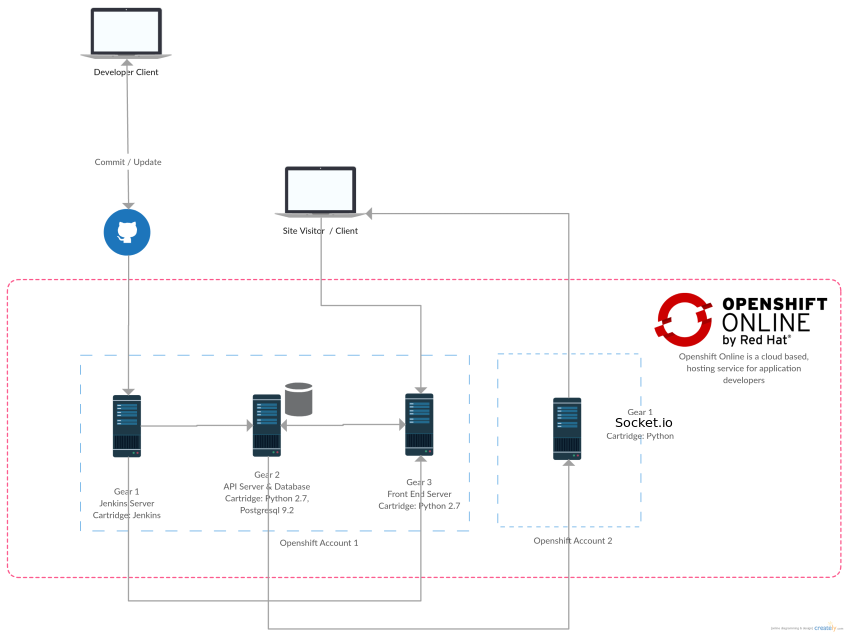
\includegraphics[width=\linewidth]{Diagrams/ArchitectureDiagram.png}
\caption{Architecture Diagram}
\label{fig:ArchDia}
\end{figure}
\section{Design Patterns}
The system shall use the AngularJS framework in the client side. The design patterns used in the development of the single page application using angularjs include the following: 


In creating directives, the composite pattern will be used in order to describe that a group of objects are to be treated in the same way as a single instance of an object. \\
Here is an example of creating a directive for a single product:
\begin{lstlisting}[basicstyle=\footnotesize,language=HTML,]
<!doctype html>
<html>
  <head>
  </head>
  <body>
    <single-product title="Zippy">
      <-- product thumbnails and details-->
    </single-product>
  </body>
</html>
myModule.directive('singleProduct', function () {
  return {
    restrict: 'E',
    template: '<div><div class="header"></div><div class="content" ng-transclude></div></div>',
    link: function (scope, el) {
      el.find('.header').click(function () {
        el.find('.content').toggle();
      });
    }
  }
});
\end{lstlisting}
In order to export the public API and resources from the server, the module pattern will be used. The module pattern  is very useful when defining services in AngularJS. Using this pattern we can simulate (and actually achieve) privacy:
\begin{lstlisting}[basicstyle=\footnotesize,frame=single,]
app.factory('foo', function () {

  function privateMember() {
    //body...
  }

  function publicMember() {
    //body...
    privateMember();
    //body
  }

  return {
    publicMember: publicMember
  };
});
\end{lstlisting}
This way, once we want to inject a function inside any other component we won't be able to use the private methods, but only the public ones. This solution is extremely powerful especially when one is building a reusable library. \\
In implementing the REST resource access, another option would be to use the Data Mapper pattern. A data mapper is used for bidirectional transfer of data between a persistent data store and an in memory data representation. The AngularJS application will communicate with the API server, which is written in Flask(Python).\\
The angular \$resource will help us communicate with the server and access our restful api. For example,
\begin{lstlisting}[basicstyle=\footnotesize,frame=single,]
API Method:
GET /api/v1/producttypes/:id

app.factory('ProductType', function ($q) {

  function ProductType(name, description) {
    this.name = name;
    this.description = description;
  }

  ProductType.get = function (params) {
    var type = $http.get('/api/v1/producttypes/' + params.id);
   
    $q.all([type])
    .then(function (type) {
      return new ProductType(type.name, type.description);
    });
  };
  return ProductType;
});
\end{lstlisting}
This way we create pseudo-data mapper, which adapts our API according to the SPA requirements. \\
We can use the User service by:
\begin{lstlisting}
function MainCtrl($scope, User) {
  User.get({ id: 1 })
  .then(function (data) {
    $scope.user = data;
  });
}
\end{lstlisting}

\chapter{SQAP} % Event Response Chart & Pentesting
\section{Abstract}
This document is about the Software Quality Assurance Plan $(SQAP)$ of the system, e-store which is an e-commerce platform for online merchants. It provides the power to grow your web business, reach more customers and sell more products and services. It enables businesses to experience an integrated workflow for their business: Sales, Inventory and Order Management and Customer Service under one platform.
\section{Introduction}
\subsection{Purpose}
The purpose of this plan is to define the e-store Software Quality Assurance (SQA) organization, SQA tasks and responsibilities; provide reference documents and guidelines to perform the SQA activities; provide the standards, practices and conventions used in carrying out SQA activities; and provide the tools, techniques, and methodologies to support SQA activities, and SQA reporting.
	
\subsection{Scope}
This plan establishes the SQA activities performed throughout the life cycle of the e-store project.

This plan shall implement a project that follows the RESTful architectural style. The project shall be developed using the Flask microframework. There will be a clear separation of concerns between the client and the server for easy maintenance and scalability.

\newpage

\subsection{List of Definitions}
\begin{table}[ht]
\centering
\begin{adjustbox}{width=1\textwidth,center=\textwidth}
\small
\begin{tabular}{| l | l |}
\hline
\textbf{Term} & \textbf{Definition} \\
\hline
ATDD 			& Acceptance Test Driven Development \\
TDD 				& Test Driven Development \\
BDD 				& Behavior-Driven Development \\
SQA 				& Software Quality Assurance \\
UML 				& Unified Modeling Language \\
ERD 				& Entity Relationship Diagram \\
MSU-IIT 			& Mindanao State University - Iligan Institute of Technology \\
REST 			& Representational State Transfer \\
FLASK 			& Web Framework \\
Python 			& Programming Language \\
SCS 				& School of Computer Studies \\ 
Sales Inventory 	& The list of items such as the goods that are in stock \\
E-commerce 		& The buying and selling of goods over an electronic network, primarily the internet \\
Customer 		& The person who transacts in the store page of the business \\
Admin 			& The owner of the products sold in the store. \\
Product 			& The items being sold in the website \\
Cart				& The list of items the customer is going to buy \\
Checkout 		& The process in which the customer is going to buy and pay the items inside the cart \\
Gherkin 			& Business Readable, Domain Specific Language that lets you describe software’s behaviour without detailing how that behaviour is implemented.\\
QAM 				& Quality Assurance Manager \\
SQAP 			& Software Quality Assurance Plan \\
SQMP 			& Software Quality Management Plan \\
PM 				& Project Manager \\
CM 				& Configuration Manager \\
AD 				& Architectural Design \\
DD 				& Detailed Design \\ 
CI 				& Configuration Items \\
UML 				& Unified Modeling Language \\
\hline
\end{tabular}
\end{adjustbox}
\caption{List of Definitions} 
\end{table}

\newpage

\subsection{List of References}
\begin{itemize}
\item $[SQAP]$ Software Quality Assurance Plan, SPINGRID team, TU/e, 0.1.3, June 2006
\item Saleh H. (2013). Javascript Unit Testing.  Packt Publishing
\item Osmani A., (2012). Javascript Learning Design Patterns
\item Zlobin G., (2013). Learning Python Design Patterns
\item Sale D., (2014). Testing Python
\item IEEE Standard for Software Quality Assurance Processes, IEEE Std 730-2014
\item Clean Code Cheat Sheet
\item Test-Driven Development, Dr. Christoph Steindl, Senior IT Architect and Method Exponent, Certified ScrumMaster
\item Best Practices, Development Methodologies, and the Zen of Python, Valentin Haenel
\item Test-Driven Development, Gary Brown
\item Detailed Design, (2006). Parametric Technology Corporation (PTC)
\item ESA Software Engineering Standards (ESA PSS-05-0 Issue 2), ESA Board for Software Standardization and Control (BSSC), 1991
\item Configuration Items, \url {http://www.chambers.com.au/glossary/configuration_item.php}
\item \url {http://flask.pocoo.org/docs/0.10/styleguide/}
\item \url {http://explore-flask.readthedocs.org/en/latest/conventions.html}
\end{itemize}

\newpage
\section{Management}
This section describes each major element of the organization that influences the quality of the software.

\subsection{Organization}
The team shall follow the agile approach, and adhere to the scrum approach in development. The team shall consist of the Scrum Master, Product Owner and the Development Team. Throughout each iteration, SQA activities should be headed by the Scrum Master who shall also serve as the Quality Assurance Manager. The team shall follow the Behaviour-driven approach in development as an extension to the Test-driven development approach. Prior to coding any functionality, the individual responsible for the feature shall create just enough acceptance tests, unit tests and code to pass the tests. 

\subsection{Tasks}
The SQA team’s main task is to check whether the procedures are followed and that standards are handled correctly as defined in the [SQAP]. Additionally, the SQA team inspects whether all group members fulfill their tasks according to the parts of the [SQAP] applying to their specific tasks. \\

Besides the described main task, the SQA team has to check the consistency and coherence between documents.

\subsection{Responsibilities}
The responsibility of Quality Assurance shall be vested in all of the members of the development team. Each one shall serve as a tester and developer at the same time. However, a Software Quality Assurance Manager (QAM) shall be the one to oversee that the BDD approach is followed, and that tests cover 100 percent coverage throughout the system, in order to avoid any bleeds or regression. The agile team shall be self-organizing individuals and take full responsibility in the feature or story assigned to them. The team shall not only be concerned with the product quality but also with the process quality and relationship between them. Should there be any major problems, the QAM shall take over and plan as needed. 

\newpage
\section{Documentation}
The documents to be delivered in the specific phases of the project will be based in Chapter 6, Section 5. Document standards are described in the same section. The Diagrams will be at Chapter 7 with the Storyboard.

\section{Standards, Practices, Conventions And Metrics}
\subsection{Documentation Standards}
Documentations may be in the form of a test, a docstring, or any formal document. If possible, the code should serve as enough documentation for the system. Throughout the project, PEP 8 style guide convention shall be used. 

\subsubsection{PEP 8 basically commands developers the following practices: }
\begin{itemize}
\item Indentation: Indent with 4 real spaces (no tabs)
\item Maximum line lenght: 79 characters with a soft limit for 84 if absolutely necessary. Try to avoid too nested code by cleverly placing break, continue and return statements.
\item Continuing long statements: To continue a statement you can use backslashes in which case you should align the next line with the last dot or equal sign, or indent four spaces.
\end{itemize}

\subsubsection{Docstrings}
All docstrings shall be formatted with reStructuredText as understood by Sphinx. Depending on the number of lines in the docstring, they are laid out differently. If it’s just one line, the closing triple quote is on the same line as the opening, otherwise the text is on the same line as the opening quote and the triple quote that closes the string on its own line:

\subsubsection{Comments}
Rules for comments are similar to docstrings. Both shall be formatted with reStructuredText. If a comment is used to document an attribute, put a colon after the opening pound sign $(\#)$. 

\subsection{Design Standards}
The system shall follow the restful-architectural style. The API backend shall be built with Flask, while the frontend (running in a different port) shall be built with AngularJS. The following table describes the API model of the project: 

\subsection{API Documentation}
\subsubsection{HTTP Status Codes}
\textbf{Success Codes}
\begin{itemize}
\item 200 OK - Request succeeded. Response included
\item 201 Created - Resource created. URL to new resource in Location header
\item 204 No Content - Request succeeded, but no response body
\end{itemize}
\textbf{Error Codes}
\begin{itemize}
\item 400 Bad Request - Could not parse request
\item 401 Unauthorized - No authentication credentials provided or authentication failed
\item 403 Forbidden - Authenticated user does not have access
\item 404 Not Found - Resource not found
\item 415 Unsupported Media Type - POST/PUT/PATCH request occurred without a application/json content type
\item 422 Unprocessable Entry - A request to modify or create a resource failed due to a validation error
\item 429 Too Many Requests - Request rejected due to rate limiting
\item 500, 501, 502, 503, etc - An internal server error occured
\end{itemize}
All 400 series errors (400, 401, 403, etc) will be returned with a JSON object in the body and a application/json content type.\\
\{ \\
“status”: “error”, \\
"message": "Not Found" \\
\}

\begin{table}[ht]
\resizebox{\textwidth}{!}{%
\begin{tabular}{llll}
\hline
\textbf{Resource}  			& \textbf{URI}      & \textbf{HTTP Method} & \textbf{Description}							\\ \hline
Inventory Module  \\ \hline
Item      				& /api/v1/items/ & GET & Retrieve all items       			\\
          					& /api/v1/items/:id & GET & Retrieve single item 			\\
          					& /api/v1/items/:id & PUT & Update item 						\\ 
          					& /api/v1/items/ & POST & Create new item 					\\ \hline
Type						& /api/v1/types/ & GET & Retrieve all item types 			\\
							& /api/v1/types/:id & GET & Retrieve all types \\ 
							& /api/v1/types/:id & PUT & Update type \\ 
							& /api/v1/types/ & POST & Create new type \\ \hline
Attribute				& /api/v1/types/:id/attributes/ & GET & Retrieve all attributes under the type id \\ 
							& /api/v1/types/:id/attributes/:id/ & GET & Retrieve single attribute under the type id \\
							& /api/v1/types/:id/attributes/ & POST & Create new attribute under the type id \\
							& /api/v1/types/:id/attributes/:id/ & PUT & Update attribute details under the type id \\ \hline
AttributeValue		& /api/v1/items/:id/attributes/ & GET & Retrieve all type-attribute pair values for each item assigned to a particular type \\ 
							& /api/v1/items/:id/attributes/:id/ & GET & Retrieve a single type-attribute pair value for an item \\ 
							& /api/v1/items/:id/attributes/:id/ & PUT & Update the type-attribute pair value \\ 
							& /api/v1/items/:id/attributes/ & POST & Create new attribute value based on the type assigned to an item \\ \hline
Image 					& /api/v1/items/:id/images/ & GET & Retrieve all images for a single item\\
							& /api/v1/items/:id/images/:id/ & GET & Retrieve single image for an item \\ 
							& /api/v1/items/:id/images/:id/ & PUT & Update image for an item \\
							& /api/v1/items/:id/images/ & POST & Create new image for an item \\ \hline
Supplier				& /api/v1/suppliers/ & GET & Retrieve all suppliers \\ 
							& /api/v1/suppliers/:id/ & GET & Retrieve single supplier \\ 
							& /api/v1/suppliers/:id/ & PUT & Update a supplier \\ 
							& /api/v1/suppliers/	& POST & Create new supplier \\ \hline
Cart \& POS Module  \\ \hline
Cart 						& /api/v1/carts/			& POST & Create new cart instance  \\ 
							& /api/v1/carts/:id/ 	& PUT &  Update Cart  \\ \hline
CartItem				& /api/v1/carts/:id/items/ & GET & Retrieve all cart items \\ 
							& /api/v1/carts/:id/items/:id/ & GET & Retrieve single cart item \\
							& /api/v1/carts/:id/items/:id/ & PUT & Update single cart item \\
							& /api/v1/carts/:id/items/ & POST & Add an item to cart \\ \hline
Order					& /api/v1/orders/ & GET & Retrieve all orders \\ 
							& /api/v1/orders/:id/ & GET & Retrieve single order \\ 
							& /api/v1/orders/:id/ & PUT & Update single order \\ 
							& /api/v1/orders/ & POST & Create new order \\ \hline
OrderItem				& /api/v1/orders/:id/items/ & GET & Retrieve all order items \\ 
							& /api/v1/orders/:id/items/:id/ & GET & Retrieve single order item \\ 
							& /api/v1/orders/:id/items/:id/ & PUT & Update single order item \\
							& /api/v1/orders/:id/items/ & POST & Add new item in order \\ \hline
Wishlist 				& /api/v1/wishlists/ & GET & Retrieve all created wishlists \\ 
							& /api/v1/wishlists/:id/ & GET & Retrieve single wishlist \\ 
							& /api/v1/wishlists/:id/ & PUT & Update wishlist \\ 
							& /api/v1/wishlists/ & POST & Create new wishlist \\ \hline
WishlistItem			& /api/v1/wishlists/:id/items/ & GET & Retrieve all items under a single wishlist \\ 
							& /api/v1/wishlists/:id/items/:id/ & GET & Retrieve single wishlist item \\ 
							& /api/v1/wishlists/:id/items/:id/ & PUT & Update wishlist item \\
							& /api/v1/wishlists/:id/items/ & POST & Add new item in wishlist  \\ \hline
User 					& /api/v1/users/ & GET & Retrieve all users \\ 
							& /api/v1/users/:id/ & GET & Retrieve single user \\
							& /api/v1/users/:id/ & PUT & Update user \\ 
							& /api/v1/users/ & POST & Create new user \\  \hline							
Group 					& /api/v1/groups/ & GET & Retrieve all groups \\ 
							& /api/v1/groups/:id/ & GET & Retrieve single group \\
							& /api/v1/groups/:id/ & PUT & Update group \\ 
							& /api/v1/groups/ & POST & Create new group \\  \hline		
							& /api/v1/groups/:id/users/ & GET & Retrieve all users under a group \\ 
							& /api/v1/groups/:id/users/:id/ & GET & Retrieve a user under a group \\
							& /api/v1/groups/:id/users/:id/ & PUT & Update a user in a group (e.g. Permission) \\
							& /api/v1/groups/:id/users/ & POST & Add a user to a group \\ \hline											
Customer 			& /api/v1/site/:id/customers/ & GET & Retrieve all customers in a site \\ 
							& /api/v1/site/:id/customers/:id/ & GET & Retrieve single customer in a site \\
							& /api/v1/site/:id/customers/:id/ & PUT & Update customer in a site \\ 
							& /api/v1/site/:id/customers/ & POST & Register new customer in site or business \\ 				
\end{tabular}
}
\caption{REST API Model}
\label{API Model}
\end{table}

\subsection{Coding Standards}
With Regards to the Coding Standards the SQA team will follow the python coding standards.

\subsection{Comment Standards}
For the Comment Standards the SQA team will follow the python commenting standards.

\subsection{Testing Standards}
The SQA team will follow the lettuce BDD and Unit testing standard. The team will also follow the Penetration Testing standard in Pentesting.

\subsection{Pentesting Plan}


\newpage
\subsection{Event Response Chart}
\begin{center}
	\begin{tabular}{ m{1.5in} | m{1.5in} | m{1.5in} }	
	\textbf{Form Control} & \textbf{Event} & \textbf{Response} \\
	\hline
	Website 				& Page Loads 			& \\
	\hline
	Sign Up Button 		& Click 					& Display Sign Up Form \\
	\hline
	User Name 			& Field Receives Focus 	& Place Cursor in User Name Field \\
	\hline
	Email 				& Field Receives Focus 	& Place Cursor in Email Field. \\ \cline{2-3}
	      				& Field Loses Focus 		& Verify if Email is Valid \\
	\hline
	Password 			& Field Receives Focus 	& Place Cursor in Password Field \\
	\hline
	Confirm Password 	& Field Receives Focus 	& Place Cursor in Confirm Password Field. \\ \cline{2-3}
						& Field Loses Focus 		& Verify if input in Confirm Password Field is the same as Password Field \\
	\hline
	Create button 		& Click 					& Verify Validity of information inside the fields. Post to the Resource '/api/v1/users/'. Display Sign In Page  	\\
	\hline
	Already Have an Account Link & Click 			& Display Sign Up Form \\
	\hline
	Forgot Your Password Link & Click 			& Display Forgot Password Form \\
	\hline 	
	Enter Email 			& Field Receives Focus 	& Place Cursor in Enter Email Field \\
	\hline
	Next Button 			& Click 					& Verify Email. Display Confirm page \\
	\hline
	No Button 			& Click				 	& Display Forget Password Form \\
	\hline
	Yes Button 			& Click 					& Send Password to Given Email. Diplay Password Sent Page \\
	\end{tabular}
	\newpage
	
	\begin{tabular}{ m{1.5in} | m{1.5in} | m{1.5in} }
	Back to Login Button & Click 				& Display Sign In Form \\ \cline{1-1}
	Sign In Button 		& 						& \\
	\hline
	Login Button 		& Click 					& Verify Fields. Log User in. Display Ladning Page \\
	\hline
	Shopping Cart Icon 	& Click 					& Verify if logged in. Display Shopping Cart Page \\
	\hline
	Continue Shopping Button & Click 				& Display Landing Page \\
	\hline 
	Product Image 		& Click 					& Display Product Page \\
	\hline 
	Browse Button 		& Click 					& Display Landing Page \\
	\hline
	Add to Cart Button 	& Click 					& POST to the Resource '/api/v1/carts/' \\
	\hline 
	Catalogue Button 	& Click 					& Display Catalogue Page \\
	\hline 
	5 Stars Icon 		& Click 					& Record Number of Stars Clicked \\
	\hline
	Category Buttons 	& Click 					& Display Target Category \\
	\hline 
	Search Box 			& Field Receives Focus 	& Place Cursor in Search Box Field \\
	\hline
	Search Button 		& Click 					& Find All Products with the same Characters on Field then Show Products \\
	\hline
	Dashboard Button 	& Click 					& Verify if User is Admin. Load Dashboard Page \\
	\hline
	Suppliers Button 	& Click 					& Display Supplier Page. GET Resource '/api/v1/suppliers/' \\
	\hline
	Customers Button 	& Click 					& Display Customer Page. GET Resource '/api/v1/customers/' \\		
	\end{tabular}

	\newpage	
	
	\begin{tabular}{ m{1.5in} | m{1.5in} | m{1.5in} }
	Orders Button 		& Click 					& Display Orders Page \\
	\hline
	Add New Suppliers Button & Click 				& Display Supplier Form. \\
	\hline
	Name 				& Field Receives Focus 	& Place Cursor in Name Field \\
	\hline
	Address 				& Field Receives Focus 	& Place Cursor in Address Field \\
	\hline
	Phone Number 		& Field Receives Focus 	& Place Cursor in Phone Number Field \\ 
	\hline
	Fax 					& Field Receives Focus 	& Place Cursor in Fax Field \\
	\hline
	Is Active 			& Field Receives Focus 	& Place Cursor on Is ACtive Checkbox \\
	\hline
	Add Button 			& Click 					& Verify the Fields. POST to a Resource uri. Display previous Page \\
	\hline
	Cancel Button 		& Click 					& Display previous Page \\
	\hline
	E-store Logo 		& Click 					& Display Dashboard Page \\
	\hline 
	Add New Order Button & Click 				& Display Order Form \\ 
	\hline
	Customer ID 			& Field Receives Focus 	& Place Cursor in Customer ID field \\
	\hline
	Payment ID 			& Field Receives Focus 	& Place Cursor in Payment ID field \\
	\hline
	Transaction Date 	& Field Receives Focus 	& Place Cursor in Transaction Date field \\
	\hline
	Shipping Date 		& Field Receives Focus 	& Place Cursor in Shipping Date field \\
	\hline
	Time Stamp 			& Option Receives Focus 	& Place Cursor in Time Stamp option \\
	\hline
	Transaction Status 	& Field Receives Focus 	& Place Cursor in Transaction Status Field \\
	\hline
	Total 				& Field Receives Focus 	& Place Cursor in Total Field \\
	\end{tabular}
	
	\newpage
	
	\begin{tabular}{ m{1.5in} | m{1.5in} | m{1.5in} }
	Unit Price 			& Field Receives Focus 	& Place Cursor in Unit Price field \\
	\hline
	Discount 			& Field Receives Focus 	& Place Cursor in Discount field \\
	\hline
	Quantity 			& Field Receives Focus 	& Place Cursor in Quantity field \\
	\hline
	Back to Store Button & Click 				& Display Landing Page \\
	\hline
	Account Button 		& Click 					& Verify if logged in. Display Account Page \\
	\hline
	Change Password Button & Click 				& Display Change Password form \\
	\hline
	Enter Password 		& Field Receives Focus 	& Place Cursor in Enter Password Field \\
	\hline
	Enter New Password 	& Field Receives Focus 	& Place Cursor in Enter New Password Field \\
	\hline
	Verify New Password 	& Field Receives Focus 	& Place Cursor in Verify New Password Field \\ \cline{2-3}
						& Field Loses Focus 		& Verfiy that Enter New Password Field and Verify New Password Field are the same \\
	\hline
	Confirm Button 		& Click 					& Verify Fields. PUT to Resource '/api/v1/users/'. Display Success Page \\
	\hline
	Click Here to go Back to Account Button & Click & Display Account Page \\
	\hline
	Wishlist Button 		& Click 					& Display Wishlist Page \\
	\hline
	Heart Icon 			& Click 					& PUT to Resource '/api/v1/wishlist/' \\	
	\end{tabular}
		
	\newpage	
	
	\begin{tabular}{ m{1.5in} | m{1.5in} | m{1.5in} }
	Social Icons & Click & Display Target Social Website \\
	\hline
	Checkout Button 		& Click 					& Display Checkout Form \\
	\hline
	Remove Button 		& Click 					& Product is Removed from Shopping Bag \\
	\hline
	First Name 			& Field Receives Focus 	& Place Cursor in First Name Field \\
	\hline
	Last Name 			& Field Receives Focus 	& Place Cursor in Last Name Field \\
	\hline
	City 				& Field Receives Focus 	& Place Cursor in City Field \\
	\hline
	State 				& Field Receives Focus 	& Place Cursor in State Field \\
	\hline
	Postal Code 			& Field Receives Focus 	& Place Cursor in Postal Code Field \\
	\hline
	Country 				& Field Receives Focus 	& Place Cursor in Country Field \\
	\hline
	Billing Address 		& Field Receives Focus 	& Place Cursor in Billing Address Field \\
	\hline
	Shipping Address 	& Field Receives Focus 	& Place Cursor in Shipping Address Field \\
	\hline
	Date Created 		& Field Receives Focus 	& Place Cursor in Date Created Field \\
	\hline
	Next Button 			& Click 					& Display Paypal Page \\
	\hline
	Continue Button 		& Click 					& Display Order Information \\
	
	\end{tabular}
	
\end{center}



\section{Review}

\section{Test}
For the tests, the SQA team will test the API's and the User Interface. For the API test refer to the Test Cases in Chapter 4 and for the User Interface Test Refer to Chapter 8. 

\section{Problem reporting and corrective actions}
If problems arise in either the Documentation or the System they need to be resolved. \\
Examples of such Problems are:
\subsection*{Document Problems}
\begin{itemize}
\item What is written and what is implemented in the system are different
\item Errors
\item Incompleteness
\item Non compliance with the Documenting Standards
\end{itemize}
\subsection*{Code Problems}
\begin{itemize}
\item Lack of functionality
\item Wrong functionality
\item Non compliance with the coding and commentary standards
\end{itemize}
\subsection*{Problem Reporting Procedure}
When a problem is detected, the person who discovered the error is responsible for reporting it to the PM and QAM. When a problem is discovered during a review, the member of the SQA team present is responsible.
\subsection*{Problem Solving Procedure}
\begin{itemize}
\item The SQA team appoints the member who is responsible for that task. He/She is responsible for solving the problem
\item When the problem is resovled the SQA team will then be notified and they will check whether the changes solved the problem
\item If the problem cannot be solved or cannot be solved within a given amount of time, the appointed member will consult with the other team members. In the consultation they will decide on what to do with the problem
\end{itemize}
\subsection{Changes in requirements of the customer}
It is also possible that the requirements of the customer change. In this case, the requested change is matched to the Charter. If the change conforms to the Charter it is accepted. If it does not conform to the Charter, the team decides wether it will discard the changes or not.

\section{Tools, techniques and methods}
The SQA team has to make sure that appropriate tools, techniques and methods are used. The tools that the team uses are:
\begin{enumerate}
\item PyCharm
\item PgAdmin 3
\end{enumerate}
These tools are readily available at \url {https://www.jetbrains.com/}

\section{Code Control}
It is the SQA teams responsibility to assure the correct handling of the code and the documents.\\
The following has to be valid:
\begin{itemize}
\item Documents are available to all people who are authorized to access them and to no one else.
\item No file is unnecessarily locked
\end{itemize}

\section{Media Control}
The SQA team will check whether all the procedures and the techniques used are handled properly.

\section{Supplier Control}
All external software components in the program code, that have an unreliable source, will be tested according to the [ESA] standards. Software components that  have reliable sources will undergo some quick tests. These tests will be focused on the parts of this software that are of importance to the project.


\section{Training}
The project requires sufficient skill in Python, Flask, and front end technologies like Angular, jQuery and Ajax. The learning curve throughout the project development has been steep and required training from the Advisor and co-team members. 

\section{Risk management}

\subsection{Categories of risks}
The following are categories of risks that are relevant to the project: 

\subsubsection{Risks with respect to the work to be done}
\textbf{1. Miscommunication} \\
\textit{Probability:} High \\
\textit{Prevention:} Daily stand ups or quick huddle should be done by the team on a regular basis. Major weekly meetings are done to keep address pressing issues in development. Team members should not hesitate to ask and re ask questions if things are unclear in order to avoid bottlenecks in the progress of the system. With regards to the customer, bi-monthly face-to-face meetups should be done to update and keep track of progress. If any confusions arise, the team may opt to use other communication mediums like phone calls, or emails to clear up problems. \\
\textit{Correction:} When it becomes clear that miscommunication is causing problems, the team members involved and the customer are gathered in a meeting to clear things up. \\
\textit{Impact:} High \\



\chapter{Diagrams}
\begin{figure}[h!]
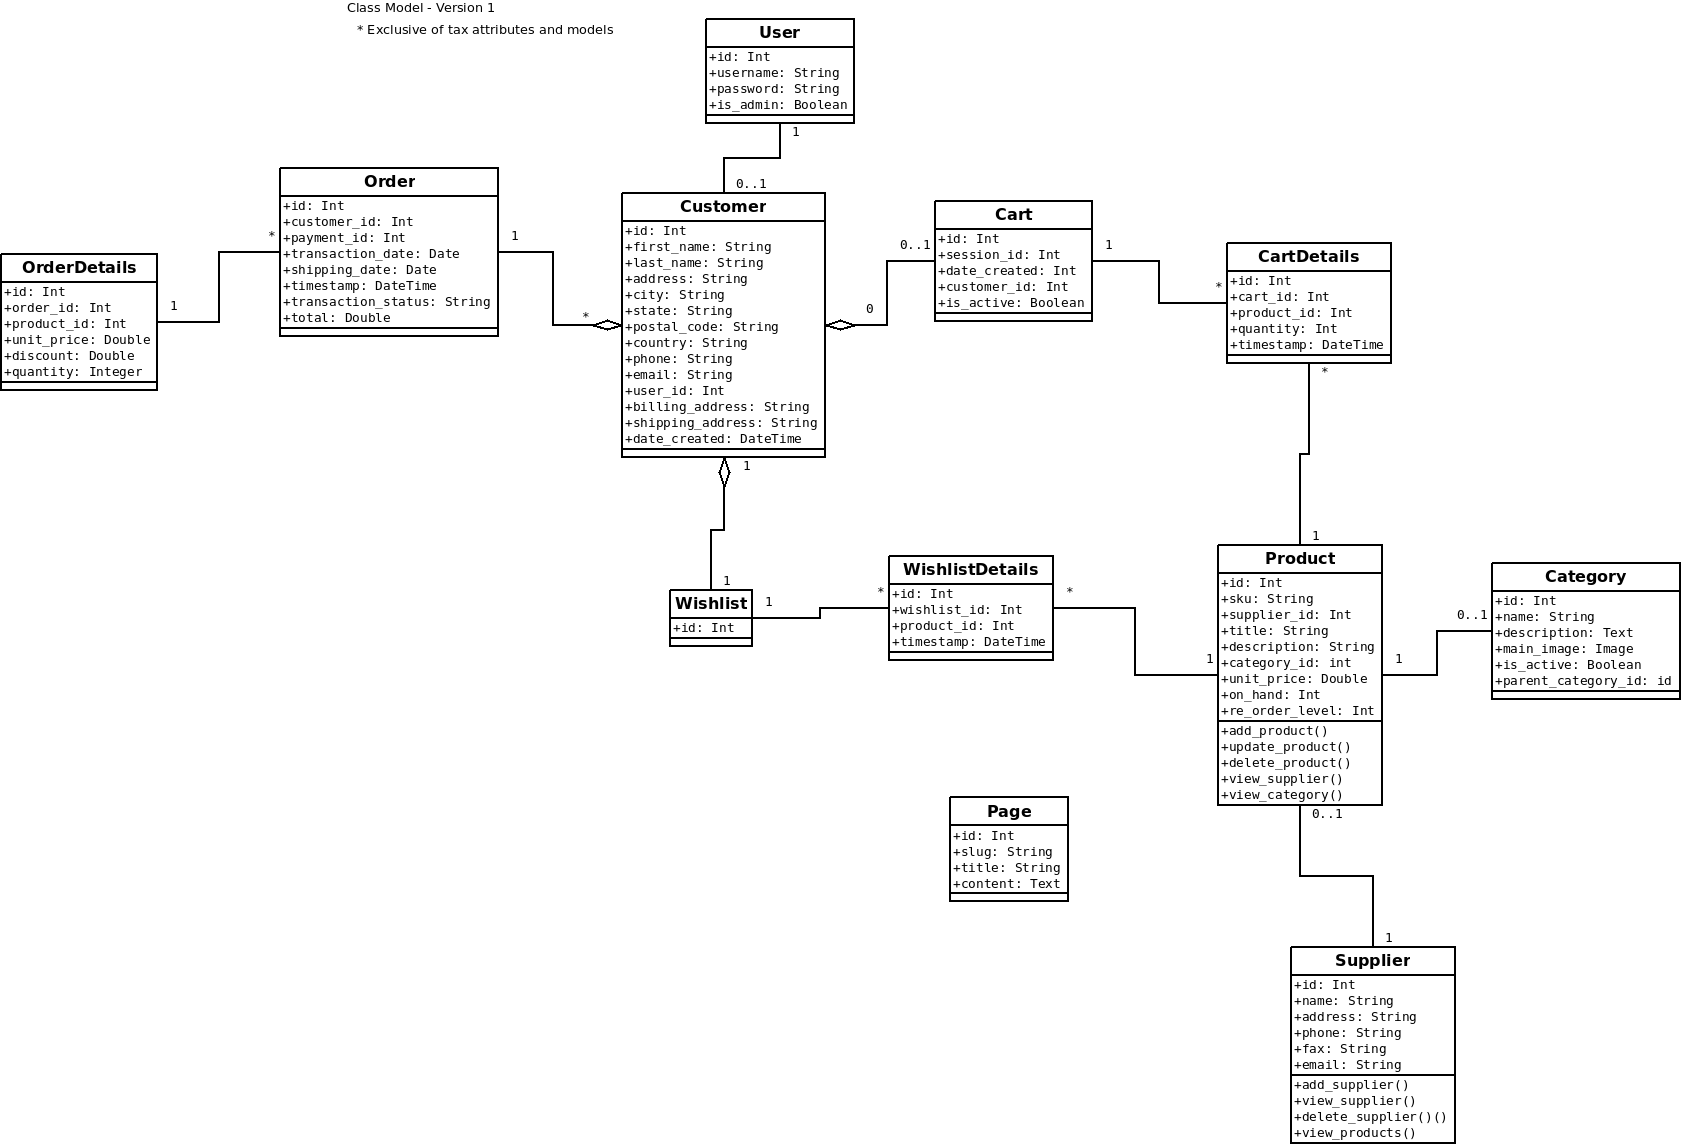
\includegraphics[width=\linewidth]{Diagrams/ClassDiagram.png}
\caption{Class Diagram}
\label{fig:ClassDiagram}
\end{figure}

\begin{figure}[h!]
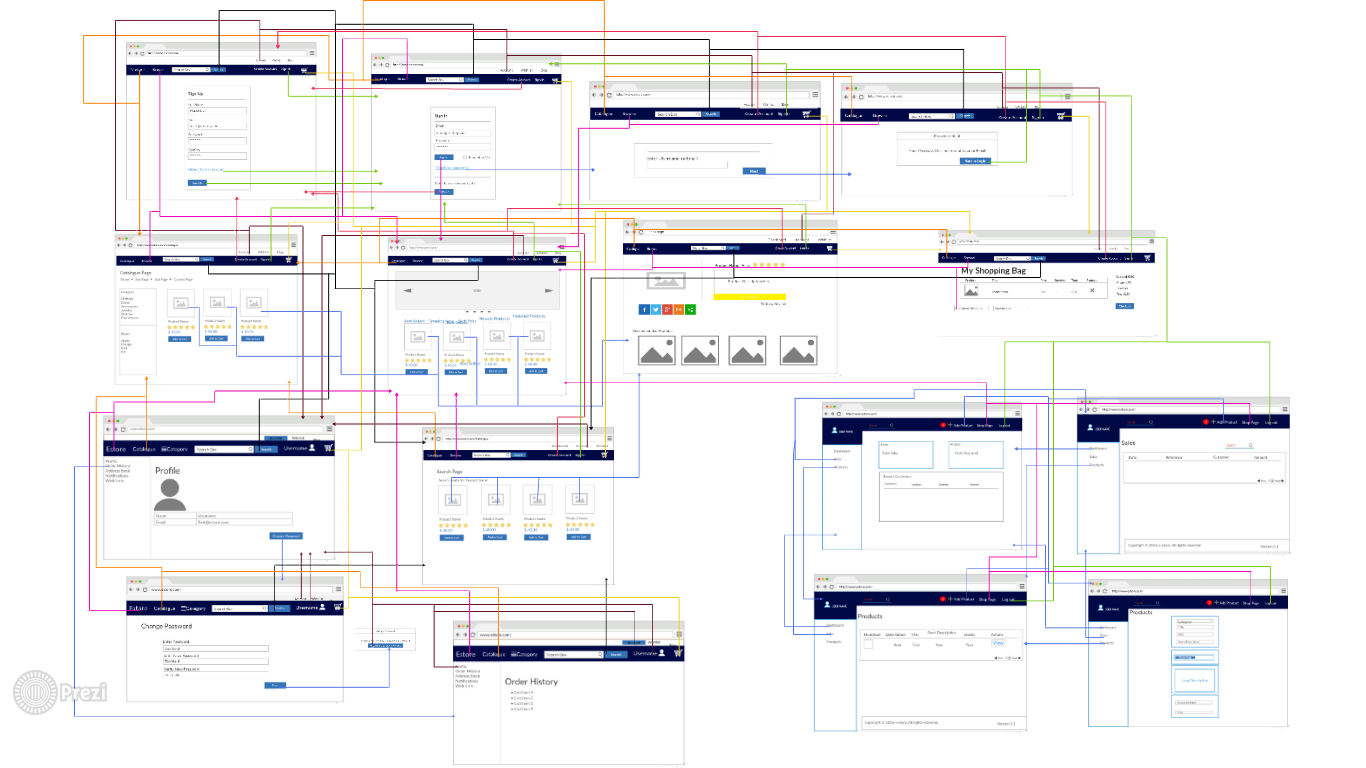
\includegraphics[width=\linewidth]{Diagrams/storyboard.png}
\caption{Storyboard}
\label{fig:Storyboard}
\end{figure}

\begin{figure}[h!]
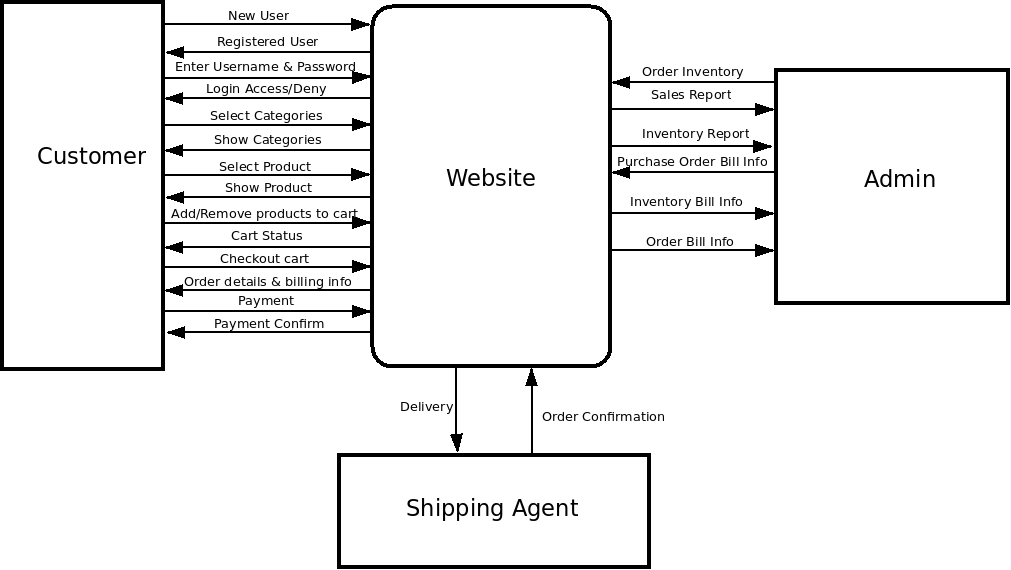
\includegraphics[width=\linewidth]{Diagrams/DataFlowDiagram.png}
\caption{Data Flow Diagram}
\label{fig:DataFlow}
\end{figure}

\begin{figure}[h!]
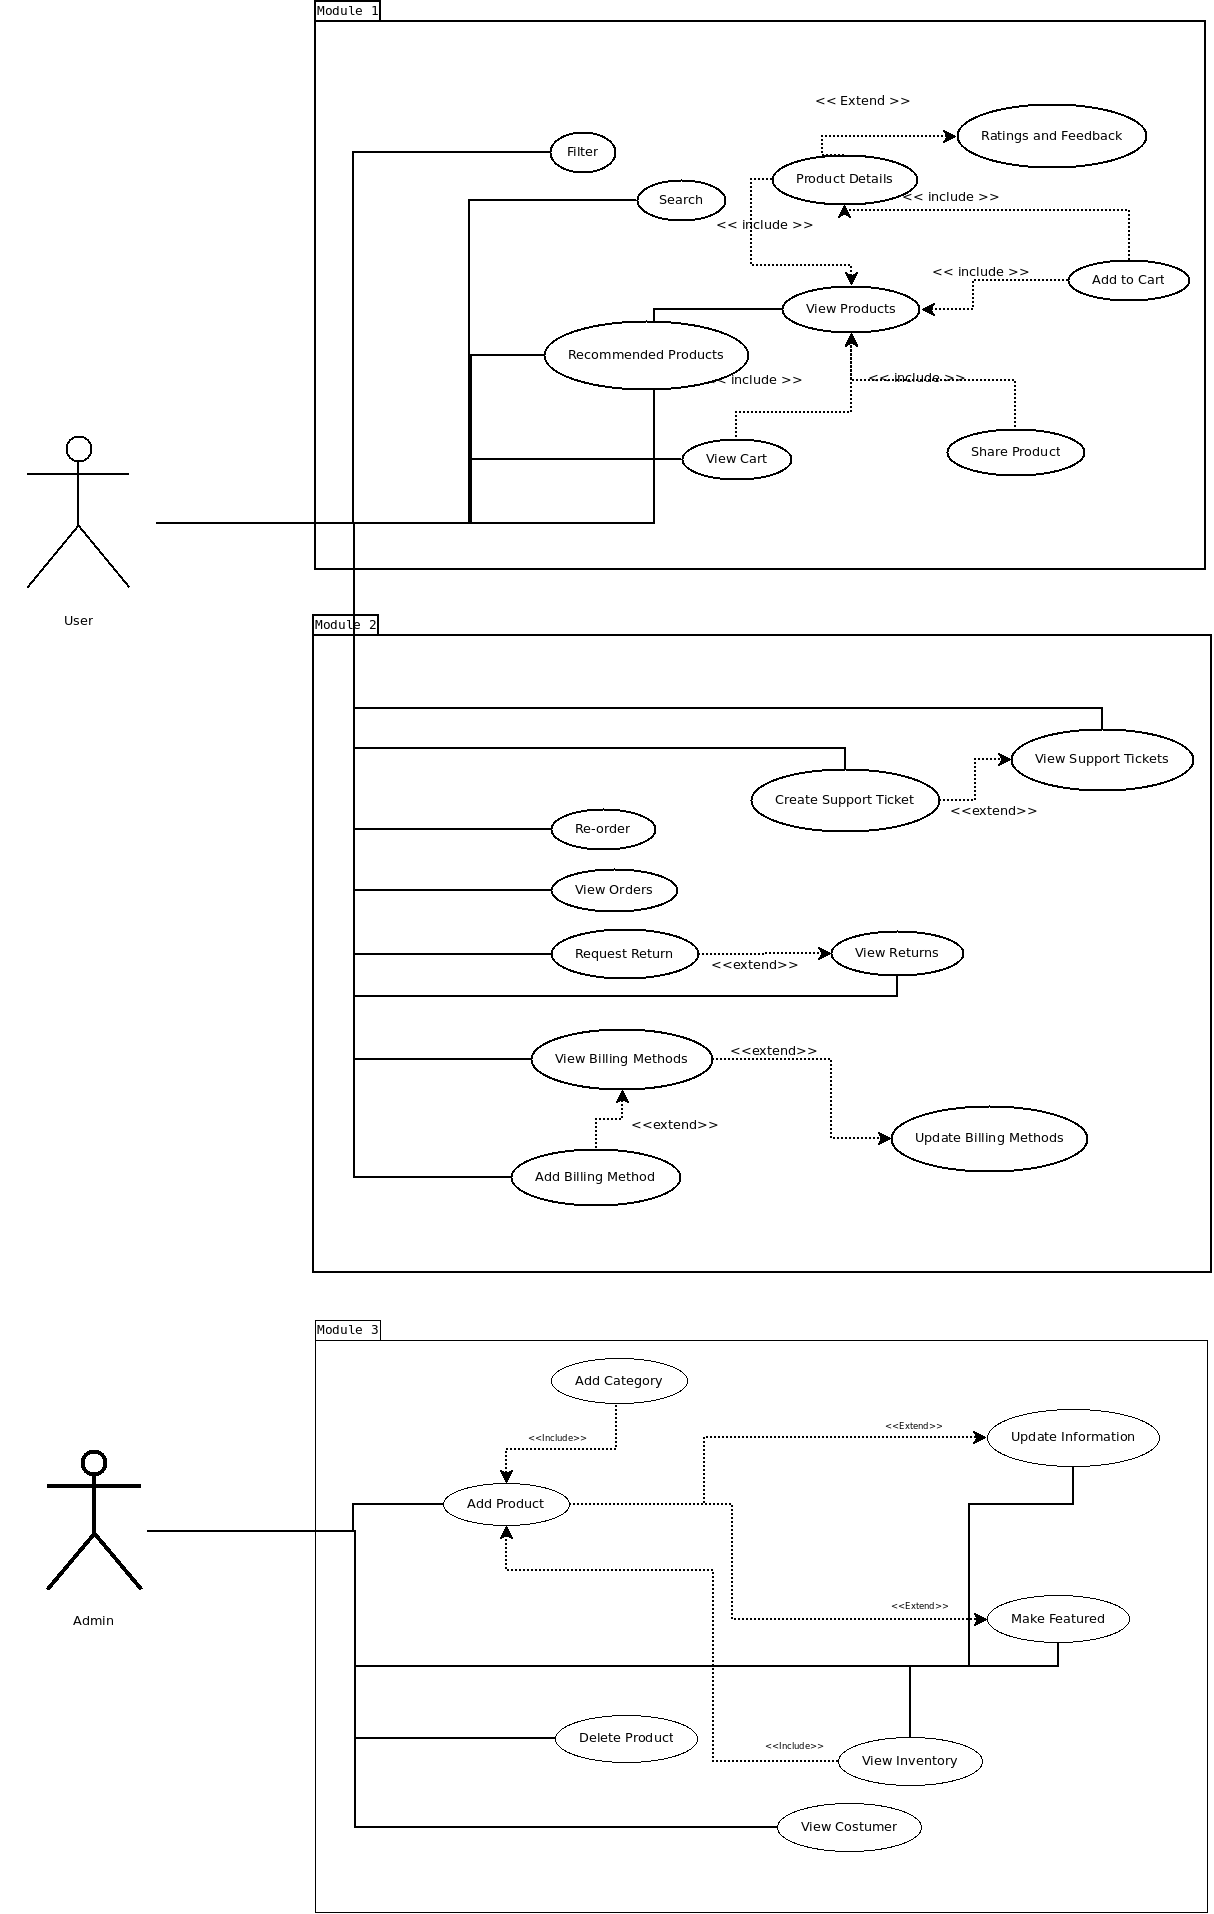
\includegraphics[width=\linewidth]{Diagrams/UseCaseDiagram.png}
\caption{Use Case Diagram}
\label{fig:UseCase}
\end{figure}

\begin{figure}[h!]
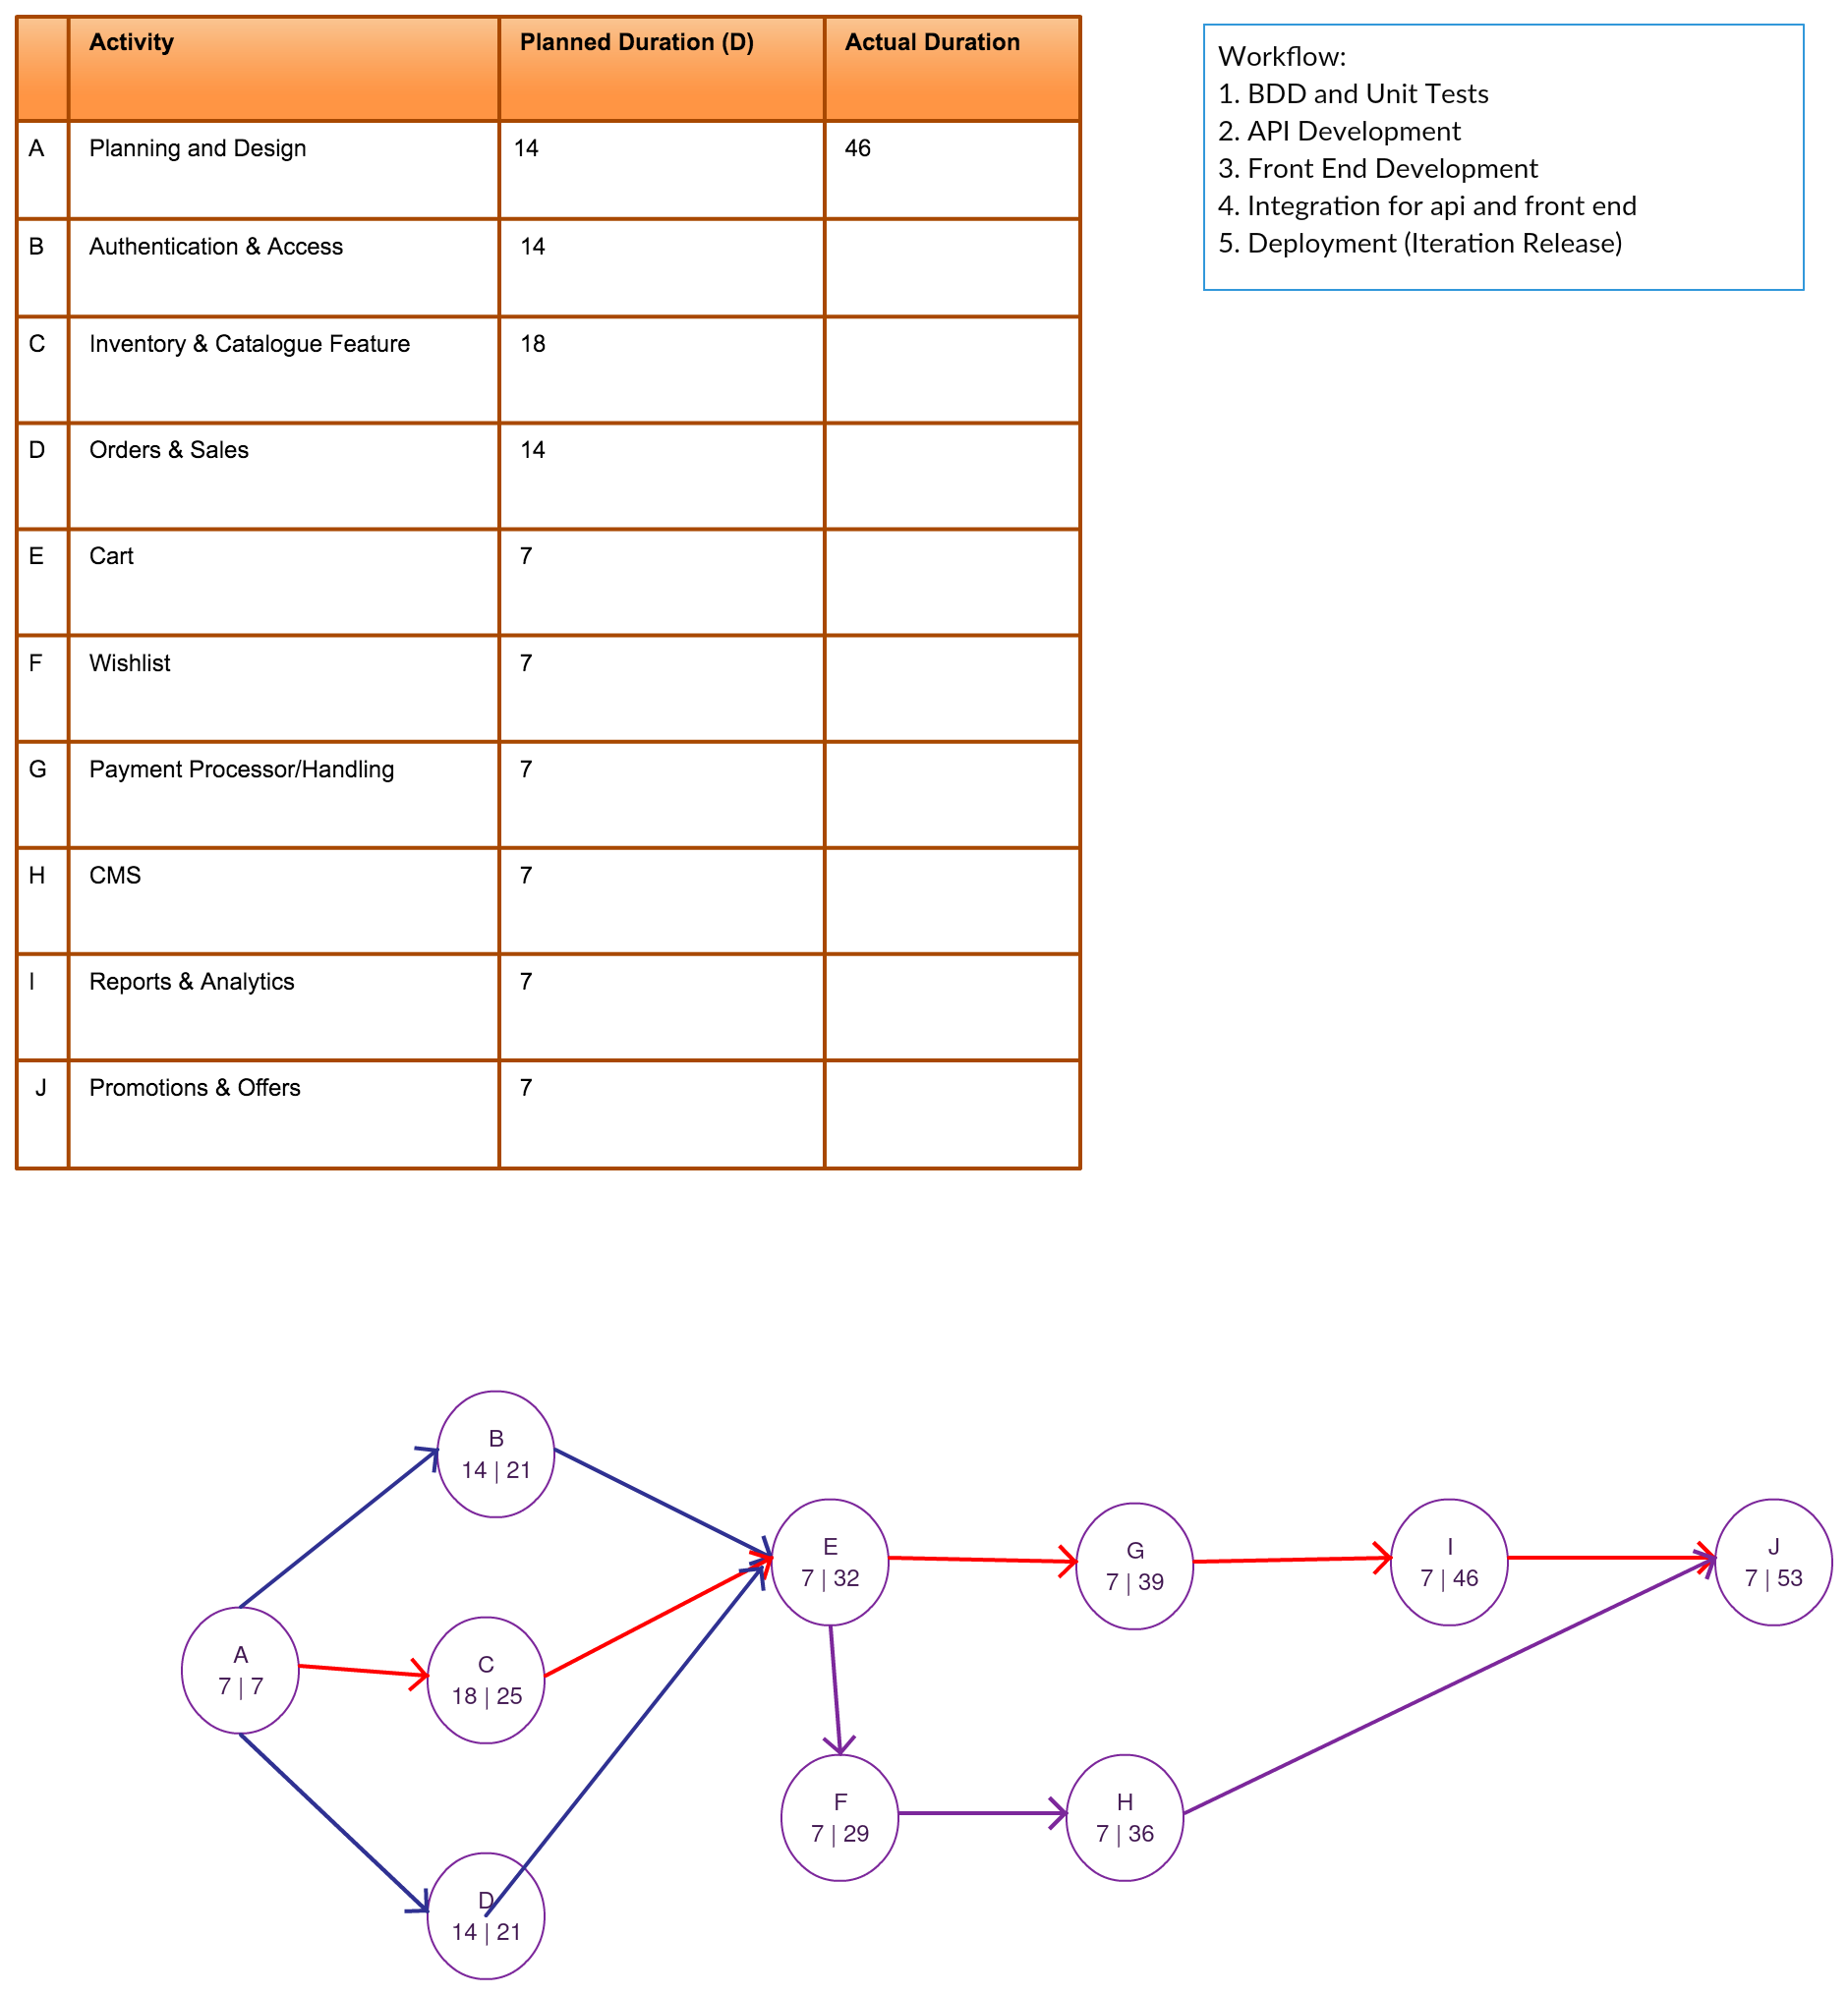
\includegraphics[width=\linewidth]{Diagrams/PertChart.png}
\caption{Pert Chart}
\label{fig:PertChart}
\end{figure}


\chapter{User Testing Results}
\section{System Usability Scale}
\begin{tabular}{ m{1.5in} m{0.4in} m{0.3in} m{0.3in} m{0.3in} m{0.4in} m{0.3in} m{0.7in} m{0.5in} }
& Strongly Disagree & & & & Strongly Agree & Scale Position & Calculation & Score Contribution \\
1. I think that I would like to use this system frequently. & $\boxdot$ & $\boxdot$ & $\boxdot$ & $\checkmark$ & $\boxdot$ & 4 & $4-1$ & 3 \\
2. I found the system unnecessarily complex. & $\boxdot$ & $\boxdot$ & $\checkmark$ & $\boxdot$ & $\boxdot$ & 3 & $5-3$ & 2 \\
3. I thought the system was easy to use. & $\boxdot$ & $\boxdot$ & $\boxdot$ & $\checkmark$ & $\boxdot$ & 4 & $4-1$ & 3 \\
4. I think that I would need the support of a technical person to be able to use this system.  & $\boxdot$ & $\checkmark$ & $\boxdot$ & $\boxdot$ & $\boxdot$ & 2 & $5-2$ & 3\\
5. I found the various functions in this system were well integrated.  & $\boxdot$ & $\boxdot$ & $\boxdot$ & $\checkmark$ & $\boxdot$ & 4 & $4-1$ & 3 \\ 
6. I thought there was too much inconsistency in this system.  & $\boxdot$ & $\boxdot$ & $\checkmark$ & $\boxdot$ & $\boxdot$ & 3 & $5-3$ & 2 \\
7. I would imagine that most people would learn to use this system very quickly.  & $\boxdot$ & $\boxdot$ & $\boxdot$ & $\checkmark$ & $\boxdot$ & 4 & $4-1$ & 3 \\
8. I found the system very cumbersome to use.  & $\boxdot$ & $\boxdot$ & $\checkmark$ & $\boxdot$ & $\boxdot$ & 3 & $5-3$ & 2 \\
9. I felt very confident using the system.  & $\boxdot$ & $\boxdot$ & $\boxdot$ & $\checkmark$ & $\boxdot$ & 4 & $4-1$ & 3 \\
10. I needed to learn a lot of things before I could get going with this system.  & $\boxdot$ & $\boxdot$ & $\checkmark$ & $\boxdot$ & $\boxdot$ & 3 & $5-3$ & 2 \\
\end{tabular}
\\
Total = 26, $Score = Total * 2.5 = 26 * 2.5 = 65$

\newpage
\section{Discussion}
The way SUS scores is:
\begin{itemize}
\item For odd items: subtract one from the user response.
\item For even-numbered items: subtract the user responses from 5
\item This scales all values from 0 to 4 (with four being the most positive response).
\item Add up the converted responses for each user and multiply that total by 2.5. This converts the range of possible values from 0 to 100 instead of from 0 to 40.
\end{itemize}
We got the scales by getting the mean of the 20 users and recorded them on the scoring form. We then do the way SUS scored it and we got the Score of 65. Having a Score of 65 means our Usability is below average since the average SUS score from all 500 studies is a 68. 

\chapter{Questionnaire}
\section{Client Questionnaire}
\begin{enumerate}
\item What kind of business is your company in?
\item What specific industries do you cater to?
\item On average, how many employees and departments do you have in your
company/business?
\item How many people at your company/business will be involved with this project?
\item How did you manage your products or inventory, manually or you're using some
applications(e.g. spreadsheets)?
\item What benefits do you expect from this project?
\item What keywords do you want people to use in search engines to find your site?
\item What are your design requirements?
\item What kinds of products will you be selling?
\item Roughly how many products will be listed on the site?
\item How would you like to organize your product?
\item Do you have product descriptions available?
\item Do you have high quality photos available for each product?
\item Do you want to allow product reviews or ratings?
\item Do you want to add social sharing icons to product pages?
\item Do you want the web site to track inventory?
\item Do you want to build an email list of customers for promotional purposes?
\item Do you offer quantity discounts?
\item Do you want to offer coupons?
\item Do you want to offer wish lists?
\item Do you have terms of service and refund policies in place for the site?
\item Would you want to integrate online payment methods in the system so that your
customers will be able to pay online? (i.e. Credit Cards, Paypal)
\item Do you have any suggested features you’d like to be implemented in the system?
\item Does this project have a deadline?
\item What is your budget for this project? Are you willing to pay?
\item Do you have anything to add?
\end{enumerate}

\chapter{References}
\url {https://bocoup.com/weblog/documenting-your-api}\\ 
\url {https://gist.github.com/iros/3426278}\\
\url {https://www.w3.org/Protocols/rfc2616/rfc2616-sec10.html} \\
\url {https://sourcemaking.com/design_patterns/flyweight} \\
\url {http://blog.rackspace.com/4-reference-architectures-to-optimize-your-ecommerce/} \\

\end{document}
